\documentclass{article}
\usepackage{amsmath}
\usepackage[utf8]{inputenc}
\usepackage{amssymb,tabu}
\usepackage{array}
\usepackage{amsthm}
\newtheorem{theorem}{Theorem}

\usepackage{parskip}
\usepackage{graphicx}
\usepackage{hyperref}
\hypersetup{
  colorlinks,
  citecolor=black,
  filecolor=black,
  linkcolor=black,
  urlcolor=black
}
\usepackage{tikz} 
\theoremstyle{definition} \newtheorem*{definition}{Definition}
\newtheorem{lemma}[theorem]{Lemma}
\newtheorem{proposition}[theorem]{Proposition}
\newtheorem*{corollary}{Corollary} \newtheorem*{remark}{Remark}
\newtheorem*{exmp}{Example} \newtheorem*{exmps}{Examples}
\newtheorem*{obvs}{Observation}

% Isomorphism symbol with function on top
\newcommand{\myiso}[1]{\stackrel{\mathclap{\normalfont\mbox{#1}}}{\cong}}
\newcommand{\dtn}{\Delta_n} \newcommand{\gene}[1]{\langle #1 \rangle}
\newcommand{\nsg}[2]{#1 \trianglelefteq #2} \newcommand{\func}[3]{#1 : #2
\rightarrow #3} \newcommand{\integers}{\mathbb{Z}}
\newcommand{\reals}{\mathbb{R}} \newcommand{\rationals}{\mathbb{Q}}
\newcommand{\naturals}{\mathbb{N}} \newcommand{\complexes}{\mathbb{C}}
\newcommand{\but}[2]{#1 \backslash \{#2\}} \newcommand{\A}{\mathcal{A}}
\newcommand{\ism}{\cong} \newcommand{\elemt}[2]{#1_{{#2}\sigma(#2)}}
\renewcommand{\vec}[1]{\mathbf{#1}}
\newcommand{\Det}[1]{|#1|}

\DeclareMathOperator{\sgn}{sgn} \DeclareMathOperator{\id}{id}
\DeclareMathOperator{\Orb}{Orb} \DeclareMathOperator{\Stab}{Stab}
\DeclareMathOperator{\Ima}{Im} \DeclareMathOperator{\Sym}{Sym}
\DeclareMathOperator{\lcm}{lcm} \DeclareMathOperator{\hcf}{hcf}
\DeclareMathOperator{\fix}{fix} \DeclareMathOperator{\ord}{\text{ord}}


\title{Algebra II} \author{John R. Britnell - 655\\ Problems class: Wednesday
2:00pm\\ Office hour: Mon 2:00pm} \date{October 2015}

\begin{document}

\maketitle

\tableofcontents \newpage

\section{Groups} 
A group is a set $G$ with a binary
operation $*$ such that \begin{itemize} \item Associativity: $(x * y)*z = x *
    (y * z)$ for all $x,y,z \in G$.  \item Identity: There is $e \in G$ such
      that $e * x = x * e$ for all $x \in G$.  \item Inverses: For all $x \in
        G$ there exists $y \in G$ such that $x * y = yz * y = e$\\
    \end{itemize}

\begin{exmps}\hfill \begin{enumerate} \item \begin{itemize} \item
            $\mathbb{Z}_n$, integers modulo $n$ under $+$.  \item $\mathbb{Z}$,
            integers under $+$.  \end{itemize} These are \emph{cyclic groups}.
      \item \begin{itemize} \item $D_{2n}$, $n \geq 3$ dihedral group (of
            rotations and reflections) of a regular $n$-gon.  \item We also
              have $D_\infty$ the \emph{infinite dihedral group}.

Take the ``polygon''.

What are the ``rotations''? These are shifts: move each vertex some number $k$
of places to the right. (if $k$ is -ve we shift left instead). 

``Reflections'' really are reflections - through a vertical axis, either
through a vertex or the midpoint of an ``edge''.

The ``rotations'' and ``reflections'' form a group under composition. This is
$D_\infty$. The subgroup of rotations is an infinite cyclic group, generated by
$R_1$

\end{itemize} \item Symmetric groups $S_n$. Permutations of $\{1, \ldots, n\}$
  under composition. $|S_n| = n!$ More generally if $\Omega$ is a set then
  $\Sym(\Omega)$, the symmetric group on $\Omega$ is the group of all
  permutations of $\Omega$.

\item Let $F$ be a field. Then $GL_n(F)$, the \emph{General Linear Group of
  degree $n$ over $F$}, is the set of \emph{invertible} $n \times n$ matrices
  with entries from $F$. It is a group under matrix multiplication.
  \end{enumerate}
  
\end{exmps}

\subsubsection*{Motivating Example}

\begin{table}[h] \centering $\begin{tabu}{l|llllll} S_3   & e     & (123) &
    (132) & (12)  & (13)  & (23)  \\ \hline e     & e     & (123) & (132) &
    (12)  & (13)  & (23)   \\ (123) & (123) & (132) & e     & (13)  & (23)  &
    (12)   \\ (132) & (132) & e     & (123) & (23)  & (12)  & (13)   \\ (12)  &
    (12)  & (23)  & (13)  & e     & (132) & (123)  \\ (13)  & (13)  & (12)  &
    (23)  & (123) & e     & (132)  \\ (23)  & (23)  & (13)  & (12)  & (132) &
    (123) & e      \\ \end{tabu}$ \end{table}

Now I want to do the Cayley table for $D_6$. We define $R$ to be the rotation,
and $U, V, W$ to be the reflections of the triangle: Then the table is:

\begin{table}[h] \centering $\begin{tabu}{l|llllll} D_6    & e      & R      &
    R^{-1} & U      & V      & W      \\\hline e      & e      & R      &
    R^{-1} & U      & V      & W      \\ R      & R      & R^{-1} & e      & V
    & W      & U      \\ R^{-1} & R^{-1} & e      & R      & W      & U      &
    V      \\ U      & U      & W      & V      & e      & R^{-1} & R      \\ V
    & V      & U      & W      & R      & e      & R^{-1} \\ W      & W      &
    V      & U      & R^{-1} & R      & e \end{tabu}$ \label{tab:cayleyd6}
\end{table} These tables coincide if we make the equivalence: $$ \begin{matrix}
  e      &\longleftrightarrow&  e \\ R      &\longleftrightarrow&  (123) \\
  R^{-1} &\longleftrightarrow&  (132) \\ U      &\longleftrightarrow&  (12) \\
  V      &\longleftrightarrow&  (13) \\ W      &\longleftrightarrow&  (23) \\
\end{matrix} $$

From an algebraic point of view these two groups are ``the same''. We say they
are \textit{isomorphic}.  \subsection{Isomorphisms} Here's a formal definition.\\


\begin{definition} Let $G$ and $H$ be groups, and let $f : G \rightarrow H$ be
a function. We say that $f$ is an \emph{isomorphism} if: \begin{enumerate}
  \item $f$ is a bijection.  \item $f(g_1 * g_2)=f(g_1) * f(g_2) $ for all
    $g_1, g_2 \in G$.

note that in $f(g_1 * g_2)$ the multiplication is happening in $g$, but in
$f(g_1) * f(g_2)$ the multiplication is in $h$. if condition (2) is satisfied,
we say that $f$ \emph{respects} $*$.

$G$ and $H$ are \emph{isomorphic} if an isomorphism $G \rightarrow H$ exists.
\end{enumerate} \end{definition}

\begin{itemize} \item $G \overset{f}{\ism} H$ if $G$ and $H$ are isomorphic and
    $f$ is the isomorphism between them.  \item $G \ism H$ if $G$ and $H$ are
    isomorhpic via some isomorphism (particular isomorphism not mentioned)
  \item $G \not\ism H$ if $G$ and $H$ are not isomorphic.\\ \end{itemize}
\begin{exmps} Determine which pairs are isomorphic:

\begin{itemize} \item $S_2=\{e, (1, 2)\}$ \item $\mathbb{Z}_2=\{0,1\}$
    operations: $+\mod 2$ \item $C_2=\{1,-1\}$ operations: multiplication
  \end{itemize} $C_n$ represents $n^{th}$ roots of unity.
  
\end{exmps}

Look at the group tables of the above:

\begin{table}[h] \centering \label{my-label} \begin{tabular}{l|ll} $S_2$  & e
    & (1,2) \\ \hline e     & e     & (1,2) \\ (1,2) & (1,2) & e
  \end{tabular} \end{table}

\begin{table}[h] \centering \label{my-label} \begin{tabular}{l|ll}
    $\mathbb{Z}_2$  & 0  & 1\\ \hline 0     & 0     & 1 \\ 1 & 1 & 0
  \end{tabular} \end{table}

\begin{table}[h] \centering \label{my-label} \begin{tabular}{l|ll} $C_2$  & 1
    & -1\\ \hline 1     & 1  & -1 \\ -1    & -1 & 1    \end{tabular}
\end{table} All groups are isomorphic, which can be shown by ``relabelling'':
\begin{table}[!hp] \centering $\begin{tabu}{rcccl} S_2  &  & \mathbb{Z}_2 & &
    C_2\\ e     & \longleftrightarrow & 0 & \longleftrightarrow & 1 \\ (1,2) &
    \longleftrightarrow & 1 & \longleftrightarrow & -1    \end{tabu}$
  \label{tab:relabelling} \end{table}


Are $\mathbb{Z}_3=\{0,1,2\}$ and $C_3=\{1,w,w^2\}$, where $w=e^{\frac{2\pi
i}{3}}$ isomorphic?

\textbf{Yes}, an isomorphism is: \begin{equation*} f : \left\{ \begin{matrix} 0
    & \mapsto & 1 \\ 1 & \mapsto & w \\ 2 & \mapsto & w^2 \\ \mathbb{Z}_3 &
    \mapsto & C_3 \end{matrix} \right.  \end{equation*}

Another: \begin{equation*} \hat{f} : \left\{ \begin{matrix} 0 & \mapsto & 1 \\
    1 & \mapsto & w^2 \\ 2 & \mapsto & w \\ \end{matrix} \right.
\end{equation*}
 
\begin{remark}\hfill \begin{enumerate} \item Let $G$ be finite and let $G \ism
        H$ then $|G|=|H|$ i.e. sets are the same size, clearly since
      isomorphism is a bijection.  \item Let $G$ have identiy $e_G$ and $H$
        have identity $e_H$. Suppose $G \ism H$. Then, $f(e_G)=e_H$.  \item
        `$\ism$' is an is an equivalence relation on groups.  We have symmetry,
      hence order does not matter for isomorphism: \begin{itemize} \item$G \ism
            G $ \textbf{(Reflexivity)} \item$G \ism H \iff H \ism G$
            \textbf{(Symmetry)} \item $G \ism H, H \ism H \implies G \ism K $
              for all groups $G,H,K$\textbf{ (Transitivity)}\\ \end{itemize}
      \end{enumerate} \end{remark}

\begin{exmp} Which of these pairs of groups are isomorphic?  \begin{itemize}
      \item $G_1 = C_4$ = $\{1,-1,i,-i\}$ \item $G_2 = $ group of
        \emph{symmetrics} (rotations and reflections) of a rectangle.\\
        Reflections: $T_x, T_y$, Rotations: $I, R_\pi$ \item $G_3 = $ Rotation
          subgroup of $D_8$.  \end{itemize}
  
Check $G_1 \ism G_3$.  \end{exmp}

\textbf{Note:} $G_1, G_3$ are cyclic groups of order 4. Let $a \in D_8$ be a
rotation of order 4.  Then $G_3 = \{e,a,a^2, a^3\}$.\hfill\\

Define a map $f:G_1 \rightarrow G_3$ by 

\begin{equation*} \begin{matrix} f(1)=e & f(-1) = a^2 \\ f(i)=a & f(-i) = a^3
  \end{matrix} \label{} \end{equation*}

\textbf{Note:} $f(i^n) = a^n$ for all $n \in \mathbb{Z}$

We can see $f$ is a bijection.

And: \begin{align*} f(i^ni^c) &= f(i^{n+c})\\ &= a^{n+c} \\ &= a^n a^c \\ &=
  f(i^n)f(i^c) \end{align*}

Hence, $f$ \emph{respects} multiplication so $G_1 \ism G_3.$\\
\begin{proposition} Let $G$ and $H$ be groups.  \begin{enumerate} \item If $|G|
        \neq |H|$ then $G$ and $H$ are not isomorphic \item If $G$ is abelian
          and $H$ is not abelian then $G \not\ism H$ \item If there exists $k
            \in \mathbb{N}$ such that $G$ and $H$ have disjoint numbers of
            elements of order $k$, then $G \not\ism H$ \end{enumerate}
      \end{proposition}

\textbf{Warning:} There does exist pairs of groups $G, H$ which passes the
three above checks but which are not isomorphic.

\begin{proof}\hfill \begin{itemize} \item Any isomorphism is a bijection.
        \item Hwk 1: if $f : G \rightarrow H$ is an isomorphism then $f(g_1)$
        commutes with $f(g_2) \iff g_1$ commutes with $g_2$ $\forall g_1,g_2
      \in G$ \item Hwk 1: If $f:G\rightarrow H$ is an isomorphism then
        $\ord(f(g))=\ord(g)$ $\forall g\in G$ \end{itemize} \end{proof}

\begin{exmps}\hfill \begin{enumerate} \item $G=S_4, H=D_8$ - Disjoint orders so
        not isomorphic.  \item $G=S_3, H=C_6=\{1,w,\ldots,w^5\}$ where
        $w=e^{\frac{2 \pi i}{6}}$\\ $H$ is abelian, but $G$ is not, so not
      isomorphic.  \item $G=C_4=\{1,i,-1,-i\}$, $H=\{I,R_\pi,T_x,T_y\}$ \\(the
        symmetry group of a rectangle). \\ Orders of $G$ are 1,4,2,4, but the
        orders of $H$ are 1,2,2,2. We have disjoint numbers of order 2,4, so
        not isomorphic.  \item $G=(\mathbb{R}, +)$, $H=(\but{\reals}{0},
          \times).$\\ -1 is an element of order 2 in $H$ but $G$ has no
          elements of order 2. Therefore not isomorphic.\\ \end{enumerate}
    \end{exmps}

\begin{proposition}\hfill \begin{enumerate} \item Let $G$ be a cyclic group of
        order $n$. Then $G \ism \mathbb{Z}_n$ \item Let $G$ be an infinite
          cyclic group. Then $G \ism \mathbb{Z}$.  \end{enumerate}
    \end{proposition}

\begin{proof}\hfill \begin{enumerate} \item Let $G=\langle g \rangle $, where
          $G$ has order $n$. Define a map $f : \mathbb{Z}_n \rightarrow G$ by
          $$f(i)=g^i \quad \text{for } i=0,\ldots,n-1$$ Clearly $f$ is a
          bijection.  \begin{enumerate} \item Suppose that $i+j<n$ for $i,j \in
              \{0,\ldots,n-1\}.$ Then $f(i+j)=g^{i+j}=g^i g^j = f(i)f(j)$.
            \item Suppose that $i+j \geq n$ The, $i+j = i+j-n$ in
              $\mathbb{Z}_n$ and $i+j-n \in \{0,\ldots,n-1\}$ so
              $f(i+j)=f(i+j-n)=g^{i+j-n}=g^{i+j}$ (since $g^n=e$).  And this is
            $g^i g^j = f(i) f(j)$.  \end{enumerate} \item Let $G=\langle g
          \rangle$ where $g$ has infinite order. Define $f : \mathbb{Z}
          \rightarrow G$ by $f(i)=g^i$ $\forall i \in \mathbb{Z}$. Clearly $f$
          is a bijection and $f(i+j)=g^{i+j}=g^i g^j = f(i) f(j)$.
      \end{enumerate} \end{proof}

\begin{remark} It follows that $\mathbb{Z}_n \ism C_n$ (complex $n^{th}$ roots
  of unity) for all $n$.  \end{remark}

\subsection{Even and odd permutations}

Consider the polynomial $\Delta_3 = (x_1 - x_2)(x_1 - x_3) (x_2 - x_3)$.  Let
$g \in S_3$, and consider the effort of applying $g$ to the variables $x_1,
x_2, x_3$ in $\Delta_3$.

$$g(\Delta_3) = (x_{g(1)} - x_{g(2)})(x_{g(1)} - x_{g(3)})(x_{g(2)} -
x_{g(3)}).$$

\noindent We see that $g(\Delta_3)=I\Delta_3$. More generally, let $$\Delta_n =
\prod_{i<j\leq n} (x_i - x_j ). $$ 

\noindent Then, if $g \in S_n$, we can apply $g$ to $\Delta_n$ by $$g(\Delta_n)
= \prod_{i<j\leq n}(x_{g(i)} - x_{g(j)}).$$

\noindent We have $g(\Delta_n) = \pm\Delta_n$.\\ \begin{definition} The
  \emph{signature} of $g$, $\sgn(g)$, is \begin{align*} +1 \quad \text{ if }
    g(\dtn) &= \dtn \\ -1 \quad \text{ if } g(\dtn) &= -\dtn \end{align*}
\end{definition}

The \emph{parity} of $g$: If $\sgn(g)=+1$, say that $g$ is \emph{even}.  If
$\sgn(g)=-1$, say that $g$ is \emph{odd}.\\

\begin{exmp}
  
In $S_3$, we have that 

$id,\,(1 2 3), (1 3 2)$ are even.

$(1 2),\, (1 3),\,(2 3)$ are odd.\\ \end{exmp} \begin{obvs}
  
The even permutations in $S_3$ form a subgroup (this always happens)\\
\end{obvs}


\begin{proposition} \label{prp:sgn}\hfill \begin{enumerate} \item
        $\sgn(gh)=\sgn(g)\sgn(h)$ for all $g,h \in S_n$.  \item
        $\sgn(g^{-1})=\sgn(g)$ for all $g \in S_n$.  \item if $\tau=(i j)$ is a
          2-cycle, then $\sgn(\tau)=-1$.  \end{enumerate} \end{proposition}

\begin{proof}\hfill \begin{enumerate} \item Let $g,h \in S_n$, \begin{align*}
              gh(\dtn) &= g(h(\dtn)) \\ &= g(\sgn(h)\dtn) \\ &=
              \sgn(h)(g(\dtn)) \\ &= \sgn(h) \sgn(g) \dtn \end{align*} So
            \begin{align*} \sgn(gh) &= \sgn(h)\sgn(g) \\ &= \sgn(g)\sgn(h)
            \end{align*}

    \item We have $g g^{-1}=e$, and clearly $\sgn(e) = +1$. 

      So $\sgn(g g^{-1})=\sgn(g)\sgn(g^{-1})=+1$ (by (1)).

      So $\sgn(g^{-1})=\sgn(g)^{-1}$ by (1).

    \item Apply $(ij)(\dtn):$ We count the number $N$ of brackets in $\dtn$
      which are sent by $(ij)$ to things of the form $(x_k - x_i)$ where $k>i$ 

      Then $\sgn\left( (ij) \right)=(-1)^N$

      Count $p,q$. $p<q$, but $(ij)(p)>(ij)(q)$

      Cases: \begin{enumerate} \item $i=p,\, j=q$ - (1 possibilty) \item
          $p=i,\,q<j$ - possibilities $q \in \left\{ i+1, \ldots, j-1 \right\}$
        \item $i<p,\,q=i$ - possibilities $p \in \left\{ i+1, \ldots , j-1
          \right\}$ \end{enumerate} So there are $2(j-i-2) +1$ possibilities in
      total.

      So $N=2(j-i-2)+1$ is odd. 

      Hence, $\sgn\left( (ij) \right)=-1$ \end{enumerate} \end{proof}

\begin{proposition} \label{prp:2cycles} Let $c=(a_1 \ldots a_r)$ be an
  $r$-cycle. Then $c$ is a product of $r-1$ 2-cycles.  \end{proposition}

\begin{proof} Easy to check that
  $$c=(a,a_n)\ldots(a,a_5)(a,a_4)(a,a_3)(a,a_2).$$ \end{proof}

\begin{corollary} An $r$-cycle is even when $r$ is odd and even when $r$ is
  even.\\ \end{corollary}

\begin{proposition}\hfill \begin{enumerate} \item Every permutation can be
        written as a product of 2-cycles.  \item If $g$ is a product of
          disjoint cycles of lengths $r_1, \ldots, r_k$

      Then the signature of $g$ is $\prod_{i} (-1)^{r_i - 1}$ \end{enumerate}
\end{proposition}

\begin{proof} We saw last year that any permutation is a products of disjoint
  cycles.

  Each of the cycles is a product of 2-cycles by Prop. \ref{prp:2cycles} and so
  $g$ is too.

  (2) Follows from Prop. \ref{prp:2cycles} and Prop. \ref{prp:sgn}.1.
\end{proof}

Rule of thumb:

A permutation is even if it has an even number of cycles of even length.

It is odd if it has an odd number of cycles of even length.\\

\begin{exmp} $$(1 2 3 4)(6 7 9)(8 4 10) \in S_{10}$$ is odd (one cycle of even
  length) \end{exmp}


\subsection{Alternating Groups}

Define $A_n=\left\{ g \in S_n | \sgn(g) = +1 \right\}$ (The even permutations
in $S_n$).\\

\begin{theorem} Let $A_n$ is a subgroup of $S_n$. If $n>1$, then
  $|A_n|=\frac{1}{2}n!$ \label{thm:subgroup} \end{theorem}

\begin{proof} $A_n$ is non-empty since it contains $e$. $A_n$ is closed under
  the group operation by Prop. \ref{prp:sgn}.1 and under inverses by Prop.
  \ref{prp:sgn}.2.

  Consider the coset $(12) A_n$. We know this coset has the same size as $A_n.$
  Since $(1 2)$ is odd, we have \begin{equation*} A_n \cap (1 2) A_n  =
    \emptyset \end{equation*}

I claim that $A_n \cup (1 2) A_n $ is $S_n$. 

Let $g \in S_n$.

If $\sgn(g) = +1$ then $g \in A_n$.  If $\sgn(g) = -1$ then $\sgn\left( (12) g
\right)= +1$.

So $(12)g \in A_n$

But $(1 2)\left( (1 2) g \right)=g$, and so $g \in (1 2)A_n$.

Hence, $|A_n|=\frac{1}{2}|S_n|=\frac{1}{2}n!$

\end{proof}

\textbf{Examples:}\\ $A_2 = \{ id \}$, $A_3 = \{id, (123), (132)\}$.

What about $A_4$? We know that $|A_4|=\frac{1}{2}4!=12$.

The cycle structures in $S_4$ are: $(1,1,1,1)$ - 1 element, $(2,2)$ - 3
elements, $(3,1)$ - 8 elements.  $A_5$ has order $\frac{1}{5}5! = 60$.

The even cycle shapes are: $(1,1,1,1,1)$ - 1 element, $(2,2,1)$ - 15 elements,
$(3,1,1)$ - 20 elements, $(5)$ - 24 elements. These four numbers add up to 60.

\emph{Exercise:} Do this for $A_6$.

\subsection{Direct products} Recall that if we have set $X_1, \ldots, X_n$, the
Cartesian product $X_1 \times X_2 \times \ldots \times X_n$ is the set of
tuples $\{(x_1, \ldots,x_n) : x_i \in X_i\}$

What if the sets are actually groups?

Let $G_1 , \ldots, G_n$ be groups. Then we can define a binary operation on
their Cartesian Product by $$(g_1, \ldots, g_n) * (h_1, \ldots , h_n) =
(g_1h_1, g_2h_2, \ldots, g_nh_n).$$ \begin{proposition} Under this binary
  operation, $G_1 \times \ldots \times G_n$ is a group. This is called the
  \textit{direct product} of $G_1 , \ldots, G_n$.  \end{proposition}

\begin{proof} Check the group axioms: \begin{itemize} \item
          \textbf{Associativity:} \begin{align*} & ((g_1, \, \ldots \, ,
            g_n)(h_1,\, \ldots, \, h_n)) (k_1, \, \ldots , \, k_n) & \\ &= (g_1
            h_1, g_2 h_2, \ldots, g_n h_n) (k_1, \ldots , k_n) & \\ &= ((g_1
            h_1)k_1, \ldots , (h_n h_n)k_n), & \text{each } G_i \text{
            associative}\\ &= (g_1, \ldots, g_n) (h_1 k_1, \ldots, h_n k_n) &
            \\ &= (g_1, \ldots, g_n) ((h_1, \ldots, h_n) (k_1, \ldots, k_n)) &
        \end{align*} \item \textbf{Identity:}

Let $e_i$ be the identity of $G_i$ for all $i$. Then $(e_1, \ldots, e_n)$ is an
identity for $G_1 \times \ldots \times G_n$ \item \textbf{Inverses:}

The element $(g_1, \ldots , g_n)$ has the inverse $(g_1^{-1}, \ldots
g_n^{-1})$.

\end{itemize}

\end{proof} \emph{Example}: Consider the group $C_1 \times C_2$ which has
elements $(1,1), (1,-1),(-1,1),(-1,-1)$

\begin{table}[h] \centering \label{my-label} $\begin{tabu}{l|llll} & e & a & b
    & c \\ \hline e & e & a & b & c \\ a & a & e & c & b \\ b & b & c & e & a
    \\ c & c & b & a & e \end{tabu}$ \end{table}

Recall the group of symmetries of the rectangle, $\{I, R_\pi, T_x, T_y\}$.

This has group table:

\begin{table}[h] \centering \label{my-label} \begin{tabular}{l|llll} & I      &
    $R_\pi$ & $T_x$   & $T_y$   \\ \hline I      & I      & $R_\pi$ & $T_x$   &
    $T_y$   \\ $R_\pi$ & $R_\pi$ & I      & $T_y$   & $T_X$    \\ $T_x$   &
    $T_x$   & $T_y$   & I      & $R_\pi$ \\ $T_\pi$ & $T_y$   & $T_x$   &
    $R_\pi$ & I     \end{tabular} \end{table}

So we have an isomorphism given by

$e \rightarrow I$\\ $a \rightarrow R\pi$\\ $b \rightarrow T_x$\\ $c \rightarrow
T_y$\\

Recall from M1P2 that $S_4$ has a subgroup $$\{id,  (12)(34)=x, (13)(24)=y,
(14)(23)=z\}.$$

This has the above group table.  \begin{table}[!ht] \centering
  $\begin{tabu}{l|llll} & id & x  & y  & z \\ \hline id & id & x  & y  & z \\ x
    & x  & id & z  & y \\ y  & y  & z  & id & x \\ z  & z  & y  & x  & id
  \end{tabu}$ \end{table}

This is also isomorphic to $C_2 \times C_2$, via $e \rightarrow id, a
\rightarrow x, b \rightarrow y, c \rightarrow z$.\\

\begin{exmp}
  
$C_2 \times C_2 \times C_2$, which has elements $(\pm 1, \pm 1, \pm 1)$. We see
there are 8 elements and $x^2=(1,1,1)=e$ for any $x$.\\ \end{exmp}

\begin{proposition}\hfill \label{prp:ordgroup} \begin{itemize} \item $|G_1
        \times \ldots \times G_n| =|G_1||G_2|\ldots|G_n|.$ \item If \emph{all}
          of the groups $G_i$ are abelian, then so is $G_1 \times \ldots \times
          G_n$. But if \emph{any} of $G_1, \ldots G_n$ is not abelian then
          netiher is $G_1 \times \ldots \times G_n$.  \item Let $(g_1, \ldots
            g_n) \in G_1 \times \ldots \times G_n$. Then $\ord (g_1, \ldots ,
            g_n) = \lcm (\ord g_1, \ldots , \ord g_n)$.  Proof not known.
        \end{itemize} \end{proposition}

\begin{proof}\hfill \begin{enumerate} \item We know from set theory that $|A
          \times B| = |A| \times |B|$ (for sets $A,B$). An easy induction shows
          that $|A_1 \times A_2 \times \dots \times A_n| = |A_1| \times |A_2|
          \times \dots \times |A_n|$.  \item Suppose that $G_1, \dots , G_n$
            are all abelian. For all $i$, let $g_i,h_i\in G_i$. Then
            $g_ih_i=h_ig_i$. Take $g,h \in G_1 \times \dots \times G_n$, say
            $g=\left( g_1, \dots , g_n \right)$, $h = \left( h_1, \dots , h_n
            \right)$. Now \begin{align*} gh &= \left( g_1 h_1, \dots , g_n h_n
              \right)\\ &= \left( h_1g_1, \dots , h_n g_n \right)\\ &= hg
            \end{align*}

For the converse, suppose that $G_i$ is not abelian for some $i$. Then there
exists $g_i,h_i \in G$ such that $g_ih_i \neq h_ig_i$. Define $g,h \in G_1
\times \dots \times G_n$ by $g = \left( e_1,\dots e_{i-1},g_ie_{i+1},\dots,e_n
\right)$ and $h = \left( e_1, \dots e_{i-1},h_i,e_{i-1},\dots,e_n \right)$
where $e_j$ is the identity of $G_j$ (or $H_j$ respectively) for all $j$. Now

\begin{align*} gh &= \left( e_1,\dots,e_{i-1},g_ih_i,e_{i+1},\dots,e_n
  \right)\\ hg &= \left( e_1,\dots,e_{i-1},h_ig_i,e_{i+1},\dots,e_n \right)
\end{align*}

So $gh \neq hg$, since they differ in the $i$th coordinate.

\item Let $g_i \in G_i$ and let $\ord g_i=h_i$ for all $i$. Let
  $m=\lcm(k_1,\dots k_n)$.

  \textbf{Fact:} $(g_1, \dots ,g_n)^{k}=(g_1^k,\dots,g_n^k)$ for all $k \in
  \integers$. (Proof: \emph{Exercise}).

  By this fact, we have \begin{align*} \left( g_1, \dots, g_n \right)^m &=
    \left( g_1^m, \dots,g_n^m \right)\\ &= \left( e_1, \dots,e_n \right)
  \end{align*} Since $k_i | m$ for all $i$.

  Suppose that $l<m$, ($l>0$). Since $m$ is the \emph{least} common multiple of
  $k_1, \dots, k_n$, we must have that $k_i\nmid l$ for some $i$. So $g_i^l\neq
  e_i$. Hence $\left( g_1^l,\dots,g_n^l \right) \neq \left( e_1,\dots,e_n
  \right)$, since they differ in coordinate $i$. So $\left( g_1 ,\dots,g_n
  \right)^l \neq \left( e_1, \dots,e_n \right)$. Hence $\ord \left( g_1
  ,\dots,g_n \right)=m$, as required.  \end{enumerate} \end{proof}

\begin{exmp} All cyclic groups are abelian, so any direct product of cyclic
  groups is abelian. For example $C_4 \times C_2$ and $C_2 \times C_2 \times
  C_2$ are ``new'' abelian groups of order 8.

  Note that these are not isomorphic, and neither of them is isomorphic to
  $C_8$. $C_8$ has an element of order 8. $C_4 \times C_2$ has an element
  $(i,-1)$ of order 4 but no element or order 8.  $C_2 \times C_2 \times C_2$
  has no element of order $> 2$.

\end{exmp} \emph{What about $C_2 \times C_4$?}

  \textbf{Observation:} For any groups $G,H$ we have $G \times H \ism H \times
  G$. An isomorphism is given by $(g,h)\mapsto (h,g)$ (routine check), so $C_2
  \times C_4 \ism C_4 \times C_2$.\\

  \begin{proposition} \label{prp:hcfcyclic} Let $m,n \in \naturals$ be such
    that $\hcf(m,n)=1$. Then $C_m \times C_n \ism C_{mn}$.  \end{proposition}

  \begin{proof} Let $C_m = \gene{g}$, $C_n=\gene{h}$. Then $\ord(g)=m$ and
    $\ord(h)=n$. So $\ord(gh)$ is $\lcm(m,n)$ by Prop. \ref{prp:ordgroup}.3.
    But $\lcm(m,n)=mn/\hcf(m,n)$ and this is $mn$ since $\hcf(m,n)=1$. So $C_m
    \times C_n$ has an element $(h,g)$ of order $mn$, so it is cyclic. Hence
    $C_m \times C_n \ism C_{mn}$.\\ \end{proof} 

  \begin{theorem}(Fundamental Theorem of Finite Abelian Groups)\hfill\\ Every
    finite abelian group is a direct product of cyclic groups.
    \label{thm:funda} \end{theorem}

  \begin{proof} Omitted.  \end{proof}

  \begin{exmps}\hfill \begin{enumerate} \item There is only one abelian group
            (up to isomorphism) of order 6. The only factorisations of 6 are 6,
            $3 \times 2$. So the only direct proposition of cyclic groups which
            have order 6 are $C_6$ and $C_3 \times C_2$. But these are
            isomorphic by Prop. \ref{prp:hcfcyclic}.  \item There are exactly
              three abelian groups of order 8 - those listed above.
          \end{enumerate} \end{exmps}

\subsection{Small groups} \begin{enumerate} \item Every group of order 1 is
    isomorphic to $\{1\}$.  \item Every group of prime order is cyclic, so
      isomorphic to $C_8$. So only one group of order $2,3,5,7,\ldots$

\item Groups of order 4: Certainly we have $C_4$. Any other group must have 3
  elements of order 2, say $a,b,c$. Start our multiplication table:

  \begin{table}[h] \centering $\begin{tabu}{l|llll} & e&a&b&c\\\hline e &
      e&a&b&c\\ a & a&e& &\\ b & b& &e&\\ c & c& & &e \end{tabu}$
    \label{tab:startedtable} \end{table}

The six vacant places are all determined by the fact that every element must
appear onee in every row and every column.

Complete table: \begin{table}[h] \centering $\begin{tabu}{l|llll} &
    e&a&b&c\\\hline e & e&a&b&c\\ a & a&e&c&b\\ b & b&c&e&a\\ c & c&b&a&e\\
  \end{tabu}$ \label{tab:completesimpletable} \end{table}

So $G \equiv C_2 \times C_2$ (So every group of order 4 is abelian).

\item Groups of order 6.

  Certainly we have $C_6$. Any other group has 5 elements with orders 2 or 3,
  with at least one of order 2 (by Prop. \ref{prp:ordgroup})

  \underline{Result:} if a group $G$ has only elements of order $\leq 2$, then
  $G$ is abelian. (If $g^2 = e$ for all $g$, look at $(ab)^2 = e$ So
  $ab\underline{ab}=e$ and also $ab\underline{ba}=aa=e$. By left cancellation,
  $ab=ba$, for all $a,b$

  The abelian groups of order 5 are $C_6, C_2 \times C_3$, which are
  isomorphic. If follows that every group of order 6 hs an element of order 3.

  Let $a$ be an element of order 3.

  Let $b$ be an element of order 2.

  \begin{equation} G = \langle a \rangle \cup b \langle a \rangle \text{ so } G
    = \left\{ e,a,a^2,b,ba,ba^2 \right\} \label{} \end{equation}

  Starting our multiplication table: \begin{table}[h] \centering
    $\begin{tabu}{l|llllll} &e   &a   &a^2  & b   &ba   &ba^2\\\hline e   &e
      &a   &a^2\\ a   &a &a^2 &  e\\ a^2    &a^2   &e    &a\\ b   &b &ba
      &ba^2& e \\ ba  &ba& ba^2& b\\ ba^2 &ba^2 &b &ba
    
  \end{tabu}$ \label{tab:multtableincomplete} \end{table}

Note that if $ab=ba$ then we can check that $ab$ must have order 6, since
$(ab)^2=a^2b^2=a^2$, $(ab)^3=a^3b^3=b.$ But $G$ is not cyclic, by assumption,
so $ab\neq ba$.  Hence we must have $ab = ba^2$.

This allows us to complete the multiplication table:

\begin{table}[h] \centering \label{my-label} $\begin{tabu}{l|llllll} & e & a &
    a^2 & b & ba & ba^2    \\ \hline e & e & a & a^2 & b & ba & ba^2    \\ a &
    a & a^2 & e & ba^2 & b & ba    \\ a^2 & a^2 & e & a & ba & ba^2 & b  \\ b &
    b & ba & ba^2 & e & a & a^2    \\ ba & ba & ba^2 & b & a^2 & e & a   \\
    ba^2 & ba^2 & b & ba & a & a^2 & e \end{tabu}$ \end{table}

We can check that  $G$ is isomorphic to $S_3$. So the groups of order 6 are
$C_6$ and $S_3$.

\item Groups of order 8.

  Abelian groups: $C_8,C_4\times C_2, C_2 \times C_2 \times C_2.$ 

  Non abelian group $D_8$.

  There is one other non abelian group.  \begin{equation*} Q_8 = \left\{ \pm1,
    \pm i, \pm j, \pm k \right\} \text{ where } i^2=j^2=k^2=-1.  \label{}
  \end{equation*} \begin{equation*} \begin{matrix} ij=k & jk=i & ki=j \\ ji=-k
      & kj=-i & ik=-j \end{matrix} \end{equation*} This is the \emph{quaternion
  group}.  $Q_8$ has six elements of order 4.  $D_8$ only has two elements of
  order 4, so they are not isomorphic.

  Alternatively, lets define matrices

  \begin{equation*} A = \left( \begin{matrix} 0 & 1 \\ -1 & 0 \end{matrix}
    \right), B = \left( \begin{matrix} i & 0 \\ 0 & -i \end{matrix} \right), C
    = \left( \begin{matrix} 0 & -i \\ -i & 0 \end{matrix} \right) \label{}
  \end{equation*}

  So $A,B,C \in GL_2(\mathbb(C))$. I claim that if $G = \left\{ \pm I, \pm A,
  \pm B, \pm C \right\}$

  Then $G \leq GL_2(\mathbb(C))$ and there is an isomorphism $G \equiv Q_8$
  given by 

  \begin{equation*} \begin{matrix} f(\pm I ) = \pm 1 & f(\pm A) = \pm i \\
      f(\pm B ) = \pm j & f(\pm C ) = \pm k \end{matrix} \label{}
  \end{equation*} It follows that since matrix multiplication is associative,
  the multiplication on $Q_8$ is associative too!

\item All groups of order 9 are abelian, so either $C_9$ or $C_3 \times C_3$.
  The groups of order 10 are $C_{10}$ and $D_{10}$. Groups of order 12 are
  $C_{12}$, $ C_{6} \times C_2$ (the abelian ones), $D_{12},A_{4}$, and one
  other. 

  Groups of order 14 are $C_{14}$ and $D_{14}$. 

  The only group of order 15 is $C_{15}$.

  There are 14 groups of order 16.  \end{enumerate}

Helpful result: \begin{proposition} Let $G$ be a group of even order. Then $G$
  has an element of order 2.  \end{proposition}

\begin{proof} Let $S$ to be the subset of $G$ such that \begin{equation*} S =
    \left\{ g \in G : \ord g > 2 \right\}.  \end{equation*} $g \in S \iff
  g^{-1} \in S$ (Since $\ord g^{-1} = \ord g$). And $g \neq g^{-1}$, since $g^2
  \neq e$. So $S$ contains pairs $(g,g^{-1})$ of elements, so $|g|$ is even. 

  But $|G|=|S| + |\left\{ g : \ord g=2 \right\}| + 1$ (identity). 

  So $|\left\{ g : \ord g = 2 \right\}|=|G|-|S|-1$ which is odd. 

  So $\left\{ g : \ord g = 2 \right\} \neq \emptyset.$

\end{proof}


\subsection{Homomorphisms}

For an isomorphism we had two conditions that a map $G \rightarrow H$ has to
satisfy:

\begin{enumerate} \item Bijection \item Respect of multiplication
  \end{enumerate}

If we drop (1), we get the definition of a homomorphism.\\

\begin{definition} A map $f:G \rightarrow H$ is a \emph{homomorphism} if $f(g_1
  g_2)=f(g_1)f(g_2)$ for all $g_1,g_2 \in G.$\\ \end{definition}

\begin{exmps}\hfill \begin{enumerate} \item Any isomorphism is a homomorphism.
        In fact an isomorphism is a bijection homomorphism.  \item Let $G,H$ be
          any groups. Then $f : G \rightarrow H$ defined by $f(g) = e_H$ is a
          homomorphism. (Check $f(g_1 g_2)=e_h$, $f(g_1)f(g_2)=e_He_h = e_h$).
          This is the ``trivial homomorphism'' $G \rightarrow H.$ \item Let $G
          \leq H$. Then $f:G\rightarrow H$ defined by $f(g)=g$ is a
        homomorphism. (The inclusion map of $G$ into $H$.) \item Define
          $\text{sign}:S_n \rightarrow C_2$ by
          $\text{sign}(g)=\text{sign}(g)=+1 \text{ if } g $ is even, $-1$ if
          $g$ is odd. (We showed before that $\sgn(gh)=\sgn(g)\sgn(h)$.) \item
            Define $f:D_{2n} \rightarrow C_2$ by 

    $f(g)=1$ if $g$ a rotation, $-1$ if $g$ a reflection.

    This is a homomorphism. (We know rot $\times$ rot $=$ rot, ref $\times$ rot
    $=$ ref, rot $\times$ ref $=$ ref, ref $\times$ ref $=$ rot).

    So its easy to see that $f$ respects multiplication.

  \item Define $f:GL_2(F) \rightarrow F^\times$ by $$F(g) = \text{det}g.$$ Then
  $f$ is a homomorphism.  (We know that
$\text{det}(gh)=(\text{det}g)(\text{det}h)$ for $g,h \in GL_2(F)$.) This can be
done for $n>2$ as well.  \item Let $V,W$ be vector spaces, and let $T:V
  \rightarrow W$ be a linear transformation. Then $V$ and $W$ are groups under
  $+$ and $T$ is a homomorphism (We know that $T(v_1 + v_2)=T(v_1)+T(v_2)$
  since $T$ preserves addition.) \item Define $f: (\mathbb{R},+)\rightarrow
    (\mathbb{C}^\times,\times)$ by $f(x)=e^{2 \pi i x}.$ Then $f$ is a
    homomorphism. (Check: $f(x+y)=e^{2\pi i (x+y)}=e^{2\pi i x}e^{2 \pi i
    y}=f(x)f(y)$).\\ \end{enumerate}
  
\end{exmps}


\begin{proposition} Let $f: G \rightarrow H$ be a homomorphism.
\begin{enumerate} \item $f(e_G)=e_H$ \item $f(g^{-1})=f(g)^{-1}$ for all $g \in
    G$.  \item $\ord f(g)$ divides $\ord g$ for all $g \in G$.  \end{enumerate}
\end{proposition}

\begin{proof} (1) and (2) are the same as for the corresponding parts of
  Proposition \ref{prp:sgn}.

  (3) \emph{Claim:} $f(g^k)=f(g)^k$ for all $k\in \mathbb{Z}.$ \begin{proof} If
    $k \geq 0$, use induction. If $k<0$, show instead that $f\left( \left(
    g^{-1} \right)^{-k} \right)=f(g^{-1})^{-k}$. (i.e. replace $g$ with
    $g^{-1}$ and $k$ with $-k$). Now suppose that $k=\ord g$. Then $g^k = e_G$.
    $f(g^k)=f(e_G)=e_H$. Now by the claim, $f(g)^k=e_H$ and so we have $\ord
    f(g)$ divides $k$.  \end{proof} \end{proof}

\begin{definition} Let $f:G \rightarrow H$ be a homomorphism. We define: 
  
  The \emph{image} of $f$: $\text{Im } f = \left\{ f(g) : g \in G \right\}$.

  The \emph{kernel} of $f$: $\text{Ker } f=\left\{ g \in G : f(g) = e_H
  \right\}$\\ \end{definition}

\begin{theorem}\hfill \begin{enumerate} \item $\text{Im } f$ is a subgroup of
        $H$.  \item $\text{Ker } f$ is a subgroup of $G$.  \end{enumerate}
      \label{} \end{theorem}

\begin{proof}\hfill \begin{enumerate} \item Check the axioms.

      $f(e_g)=e_H$ so $e_H \in \text{Im }f$.  Suppose $h_1, h_2 \in \text{Im }
      f$. Then there exist $g_1, g_2 \in G$ such that $f(g_1)=h1, f(g_2)=h_2$.
      Now, $f(g_1 g_2)=f(g_1)f(g_2)=h_1 h_2$. So $\text{Im }f$ is closed under
      the group operation.

      Suppose $h \in \text{Im }f. $ Then $h=f(g)$ for some $g \in G$. Now
      $f(g^{-1})=f(g)^{-1}=h^{-1}$. So $\text{Im }f$ is closed under inverses.
      So $\text{Im } f \in H $.

    \item Again, check the subgroup conditions.  $f(e_G)=e_H$, so $e_G \in
      \text{Ker }f$. Suppose $g_1, g_2 \in \text{Ker }f$. Then
      $f(g_1)=f(g_2)=e_H$. ow $f(g_1 g_2)=f(g_1)f(g_2)=e_He_H=e_h$. So $g_1 g_2
      \in \text{ker }f$. Finally, let $g \in \text{Ker }f$. Then $f(g)=e_H$.
      now $f(g^{-1})=f(g)^{-1}=e_H^{-1}=e_H$, so $g^{-1} \in \text{ker }f$. So
      $\text{ker }f \leq G$.  \end{enumerate} \end{proof}

\begin{exmp} Suppose $G=S_3$. Let $f$ be a homomorphism from $G$ to some group
  $H$. What are the possibilities for $\text{Im }f$ and $\text{Ker }f$?

  Recall that for $g \in G$ we have $f(g)$ divided $\ord g$.

  In $S_3$ we have elements $(123)$, $(12)$ of orders 3 and 2 respectively. So
\begin{enumerate} \item $f\left( (123) \right)$ has order 3 or else $f\left(
    (123) \right)=e_H$ \item $f\left( (12) \right)$ has order 2 or else
      $f\left( (12) \right)=e_H$ \end{enumerate}

  \textbf{Case 1:} $f\left( (123) \right)$ has order 3 and $f\left(
  (12)\right)$ has order 2. In this case $|\text{Im }f|$ is divisible by both 2
  and 3. But $|\text{Im }f| \leq 6$, so we must have $\text{Im } f=6$. So
  (considered as a map $G \rightarrow \Ima f$) $f$ is bijective. Hence $\Ima f
  \cong S_3$.

  \textbf{Case 2:} $f\left( (12) \right)=e_H$. In this case observe that
  $(123)=(13)(12)$.

  So $f\left( (123) \right)=f\left( (13) \right)e_H=f\left( (13) \right)$.

  But $f\left( (123) \right)$ divides 3 and $f\left( (13) \right)$ divides 2.
  Hence these must both be $e_H$. Now we see that $\ker f$ is a subgroup of
  $S_3$ containing $id, (123), (12), (13)$, so $\ker f=S_3$. And so $\Ima f =
  \left\{ e_H \right\}$. $f$ is the trivial homomorphism.

  \textbf{Case 3:} $f\left( (12) \right)$ has order 2, $f\left( (123)
  \right)=e_H$. Notice that $(13)(12)=(123)$, so $f\left( (13) \right)f\left(
  (12) \right)=e_H$. So $f\left( (13) \right)=f\left( (12) \right)^{-1}=f\left(
  (12) \right)$ (Since $f\left( (12) \right)$ has order 2).

  Similarly $(12)(23)=(123)$, so $f\left( (12) \right)=f\left( (23) \right)$.
  Hence the image is $\left\{ e_H,f\left( (12) \right) \right\}$, a group of
  order 2, and $\ker f=\left\{ e,(123),(132) \right\}$.

  If we take $\Ima f$ to be $C_2$, then $f$ is the sign homomorphism.\\
  \begin{obvs}
  
  Not every subgroup of $S_3$ occurred as the kernel of a homomorphism.
\end{obvs} \end{exmp}

The next subsection explores which subgroups can occur.

Suppose $\func{f}{G}{H}$ is a homomorphism, and suppse $g \in \ker f$. Let
$g_1$ be every element of $G$. Then I claim $g_1,g_0,g_1^{-1}\in \ker f$.

Check: \begin{align*} f(g_1\,g_0\,g_1^{-1}) &= f(g_1)f(g_0)f(g_1)^{-1}\\ &=
  f(g_1)e_Hf(g_1)^{-1} \\ &= e_H.  \end{align*}

So if $K=\ker f$, then $K=gKg^{-1}=\left\{ gKg^{-1} : k \in K \right\}$ for all
$g \in G.$\\

\begin{proposition} \label{prp:tfae} Let $G$ be a group and let $H$ be a
subgroup of $G$. The following are equivalent: \begin{enumerate} \item
    $H=gHg^{-1}$ for all $g \in G$.  \item $Hg=gH$ for all $g \in G$.  \item
      Every left coset is a right coset \item Every right coset is a left coset
      \item $gHg^{-1} \subseteq H$ for all $g \in G$ \end{enumerate}
  \end{proposition}

\begin{proof}\hfill \begin{itemize}

    \item[$(2) \implies (3)$:] Suppose that $Hg=gH$ for all $g$. Then if we
      take a left coset $gH$ then this is equal to the right coset $Hg$.

\item[$(3)\implies(2):$] Suppose that every left coset of $H$ is a right coset.
  So for $g \in G$, $gH=Hx$ for some $x \in G$. But $g \in gH$, and so $g \in
  Hx$. Hence $Hx=Hg$, so $gH=Hg$.

\item[$(2)\implies(4):$] The same as above.

\item[$(1)\implies(2):$] Consider $x \in gHg^{-1}$. So $x=ghg^{-1}$ for some $h
  \in H$. Now $xg=gh$. So $(gHg^{-1})g=\left\{ (ghg^{-1}) g \right\}=\left\{ gh
  : h \in H \right\}. $ $gHg^{-1}=H$, so $(gHg^{-1})g=Hg$ Hence $Hg = gH$.

\item[$(2)\implies(1):$] Suppose that $Hg=gH$. Then $Hgg^{-1}=gHg^{-1} \implies
  H=gHg^{-1}$.

\item[$(1) \implies (5):$] Since $gHg^{-1}=H \implies gHg^{-1} \subseteq H$.

\item[$(5) \implies (1):$] Supppse that $gHg^{-1}\subseteq H$ for all $g \in
  G$. Fix an element $g$. Then $g^{-1} \in G$ and so $g^{-1}H\left( g^{-1}
  \right)^{-1} \subseteq H$, so $g^{-1}Hg \subseteq H$. So $g\left( g^{-1}Hg
  \right)g^{-1} \subseteq gHg^{-1}$, and it follows that $H \subseteq
  gHg^{-1}$. But we know that $gHg^{-1} \subseteq H$, and so $H=gHg^{-2}$.
  \end{itemize} \end{proof}

\begin{definition} A subgroup $H$ of a group $G$ with the property that
  $gHg^{-1}=H$ for all $g \in G$ (or any of the other equivalent properties
  from Prop. \ref{prp:tfae}) is said to be a \emph{normal} subgroup of $G$. We
  write $H \trianglelefteq G$ to mean that it is a normal subgroup.\\
\end{definition}

\begin{exmp}\hfill \begin{enumerate} \item Every group $G$ has normal subgroups
          $\left\{ e \right\}$ and $G$. (Easy to see that $g\left\{ e
          \right\}g^{-1}=\left\{ geg^{-1} \right\}=\left\{ gg^{-1}
        \right\}=\left\{ e \right\}).$

      And for $g \in G$, $gG = G=Gg$, so $gGg^{-1}=G$ by condition $(2)$ from
      Prop. \ref{prp:tfae}.

    \item If $G$ is abelian then every subgroup of $G$ is normal. 

      (Let $H \leq G$, and let $g \in G$. Then $gH=\left\{ gh:h \in H
      \right\}=\left\{ hg:h \in H \right\}=Hg$).

    \item Let $\nsg{A_n}{S_n}$. Let $g \in S_n$, and let $h \in A_n$. Then
      $\sgn \left( ghg^{-1} \right)=\sgn(g)\sgn(h)\sgn(g)^{-1}=\sgn(h)=+1$.

      So $gHg^{-1} \in A_n$ for all $h \in A_n$. Hence $gA_ng^{-1} \subseteq
      A_n$ for all $g$ and this condition $(5)$ from Prop. \ref{prp:tfae}.

      \begin{enumerate} \item More generally, if $|G:H|=2$ (index 2 -  so $G =
            H \cup Hg$ for some $g \in G$) then $\nsg{H}{G}$. We see that the
            left cosets are $H$ and $gH$, so every left coset is a right coset.
        \end{enumerate}

    \item Let $G = D_{2n}$, and let $R$ be the rotation subgroup. Then
      $|G:R|=2$, so $\nsg{R}{G}$. In fact every subgroup of $R$ is normal in
      $G$.

      $R$ is cyclic, say $R = \langle r \rangle$.  A subgroup of $R$ is
      $\gene{r^k}$ for some $k$. Let $g \in D_{2n}$. If $g$ is a rotation then
      $g\gene{r^k}=g\left\{ r^{kl}:l \in \mathbb{Z} \right\}=\left\{ gr^{kl}:l
      \in \mathbb{Z} \right\}= \left\{ r^{kl}:l \in \mathbb{Z}
    \right\}=\gene{r^k}g$, since any two rotations in $D_{2n}$ commute.

      If $g$ is a reflection then $$g\gene{r^k}=\left\{ gr^{kl}:l \in
      \mathbb{Z} \right\}=\left\{ r^{-kl}g:l \in \mathbb{Z}
    \right\}=\gene{r^k}g,$$ since $ba=a^{-1}b$ for any rotation $a$ and
    reflection $b$ in $D_{2n}$. So in either case the left and right cosets are
    the same.

    \item $G \times H$ has a subgroup  $G \times \left\{ e_H \right\}$
      isomorphic to $G$. Call this $\hat{G}$. Then $\nsg{\hat{G}}{G \times H}$.
      \begin{align*} (g,h)\hat{G}(g^{-1},h^{-1}) &= g^{-1}Gg^{-1} \times
        h\left\{ e_H \right\}h^{-1} \\ &= G \times \left\{ e_H \right\} =
        \hat{G} \end{align*} Since $\nsg{G}{G}$, and $\nsg{\left\{ e_H
      \right\}}{H}$.

\item $V_4 = \left\{ id,(12)(34), (13)(24),(14)(23) \right\} \trianglelefteq
  S_4$. (Check that the right and left cosets are equal.) \end{enumerate}
  \end{exmp}

\subsubsection*{Non-examples} \begin{enumerate} \item $\gene{(12)}=\left\{ id,(12)
      \right\}$ in $S_3$ is not normal.

    $(13)\left\{ id, (12) \right\}=\left\{ (13),(123) \right\} \neq \left\{
    id,(12) \right\}(13) = \left\{ (13)(132) \right\}$.

  \item If $t$ is a reflection in $D_{2n}$, then $\gene{t}=\left\{ id,t
    \right\}$ is not normal in $D_{2n}$. (Assume $n \geq 3$)

    Take $g$ a rotation of maximal order. Then $$g\gene{t}=\left\{ g,gt
    \right\}=\left\{g,tg^{-1}\right\}\neq \left\{ g,tg \right\}=\gene{t}g$$
\end{enumerate}

\begin{proposition} Let $\func{f}{G}{H}$ be a group homomorphism. Then $\ker f
  \trianglelefteq G$.  \end{proposition}

\begin{proof} Let $K = \ker f$, and let $k \in K$. For $g \in G$, we have
  \begin{align*} f(ghg^{-1})=f(g)f(h)f(g)^{-1} &= f(g)e_Hf(g)^{-1} \,, k \in
    \ker f\\ &= f(g)f(g)^{-1} = e_H \end{align*}

  So $gkg^{-1} \in K$ for all $g \in K$, $k \in K$, so $gKg^{-1} \subseteq K$
  for all $g \in G$. This is condition (5) from Prop. \ref{prp:tfae}, so $K
  \trianglelefteq G$.  \end{proof}

\subsection{Quotient Groups} Let $G$ be a group, and let $H$ be a subgroup. Look
at the left cosets $\left\{ gH:g\in G \right\}$ of $H$ in $G$. Notice that
$\left\{ gH:g\in G \right\}$ is a set, where elements are cosets.

I want to try to give $\left\{ gH:g\in G \right\}$ a group structure. What is
the obvious way of defining $(g_1 H)(g_2 H)$? All we have available is
multiplication in $G$, so we try defining \[ (g_1 H )(g_2 H) = g_1 g_2 H.  \]

What possible problem is there? 

Well, if $g_1 H=g_1'H$, and $g_2 H=g_2' H$, then we need to know that \[ g_1g_2
H = g_1' g_2' H.  \]

Otherwise our multiplication will not be well-defined.

This might or might not be true.\\

\begin{exmp} Take $G = S_3$. $H = \left\{ id, (12) \right\}$.

  Cosets $id\, H=(12)H=H$, $(13)H=(123)H$, $(23)H=(132)H$.

  Now $(13)(23)=(123)$, but $(123)(132)=id$.

  So our intended definition doesn't work here, since we'd have \[
  ((123)H)((132)H)=((13)H)(\left( 23 \right)H)=(123)H \neq id\,H.  \] This is a
  contradiction.\\ \end{exmp}

\begin{proposition} If $H \trianglelefteq G$, then the definition of coset
  multiplication above is well-defined.  \end{proposition}

\begin{proof} Suppose $H \trianglelefteq G$, then $gH=Hg$ for all $g \in G$.

  Now suppose $g_1H=g_1'H$, $g_2H=g_2'H$.

  Then $g_1' = g_1h_1$, $g_2'=g_2h_2$, for some $h_1,\,h_2 \in H$.

  $g_1'g_2'=g_1(h_1g_2)h_2$. Now $h_1g_2 \in Hg_2$, and $Hg_2=g_2H$, so
  $h_1g_2=g_2h_3$ for some $h_3 \in H$. So $g_1'g_2'=g_1g_2h_3h_2 \in g_1g_2H$.
  So \[ g_1'g_2'H = g_1g_2H.  \] \end{proof}

\begin{definition} Let $G$ be a group, and $N$ a normal subgroup of $G$. Then
  $\frac{G}{N}$ is the set of all cosets of $N$ in $G$, With multiplication
  given by $(g_1N)(g_2N)=g_1g_2N$. This is the \emph{quotient} of $G$ by $N$.\\
\end{definition}

\begin{proposition} Let $N \trianglelefteq G$. Then $\frac{G}{N}$ is a group.
\end{proposition}

\begin{proof}\hfill \begin{itemize} \item (Associativity:) Let $g_1,g_2,g_3 \in
          G$.  Then \begin{align*} ( (g_1N)(g_2N))(g_3N) &= (g_1g_2N)(g_3N) \\
            &= (g_1g_2)g_3N=g_1(g_2g_3)N \quad \text{Since } G \text{ is
            associative.)}\\ &= (g_1N)(g_2g_3N)\\ &=(g_1N)\left( (g_2N)(g_3N)
          \right).  \end{align*} So $\frac{G}{N}$ is associative.  \item
          (Identity:) Let $e$ be the identiy in $G$. Then \begin{align*}
            (eN)(gN)=egN=gN \end{align*} and \begin{align*} (gN)(eN)=geN=gN
          \end{align*} for all $g \in G$.

\item Inverses: Let $g \in G$ Then \begin{align*} (gN)(g^{-1}N) = gg^{-1} = eN
    \\ (g^{-1}N)(gN) = g^{-1}gN = eN \end{align*} so $g^{-1}N$ is an inverse
  for $gN$ in $\frac{G}{N}$.  So $\frac{G}{N}$ is a group.  \end{itemize}
  \end{proof}

\textbf{Remember:} $\big|\frac{G}{N}\big|$ = number of  cosets of $N$ in $G$
whenever $G$ is a finite group.\\


\begin{exmps}\hfill \begin{enumerate} \item $A_n \trianglelefteq S_n$. The
          cosets of $A_n$ in $S_n$ are $\left\{ A_n , (12)A_n\right\}$, so
          $\big|\frac{S_n}{A_n}\big|$ has order 2. We have $A_nA_n = A_n$,
          $(12)A_nA_n=(12)A_n$, $A_n(12)A_n=(12)A_n$, $(12)A_n(12)A_n=A_n$.

      Notice that we can interpret e.g. $A_n(12)A_n$ as a set $\left\{
      g_1(12)g_2 : g_1,g_2 \in A_n \right\}$. In this case all of the
      identities above are true.

    \item For any group $G$, $G \trianglelefteq G$. Here we have
      $\frac{G}{G}=\left\{ G \right\}$, a group of size 1.

      Also, $\left\{ e \right\} \trianglelefteq G$, and $\frac{G}{\left\{ e
      \right\}}=\left\{ g\left\{ e \right\}:g \in G \right\}$, which has the
      same size as $G$. Notice that the map $\phi : G \rightarrow
      \frac{G}{\left\{ e \right\}}$ defined by $g \overset{\phi}{\mapsto}
      g\left\{ e \right\}=\left\{ g \right\}$ is an isomorphism, since $g_1g_2
      \overset{\phi}{\mapsto} \left\{ g_1g_2 \right\}=g_1g_2\left\{ e
      \right\}=(g_1\left\{ e \right\})(g_2\left\{ e
      \right\})=\phi(g_1)\phi(g_2)$. 


\newpage \item Let $G=D_{2n}$ and let $E = \gene{g}$ be the rotation subgroup.
  Then $R \trianglelefteq D_{2n}$. Now $\frac{D_{2n}}{R}=\left\{ R,tR
  \right\}$, where $t$ is a reflection.

      So $\frac{D_{2n}}{R}$ is a group of order 2.

      \begin{table}[h] \centering $\begin{tabu}{l|ll} & R & tr \\\hline R & R &
          tr \\ tr & tr & R \end{tabu}$ \label{tab:d2ntable} \end{table} or in
      other words

      \begin{table}[h] \centering \begin{tabular}{l|ll} & Rotation &
          Reflection\\\hline Rotation & Rotation & Reflection\\ Reflection &
          Reflection & Rotation.  \end{tabular} \label{tab:rottable}
      \end{table}

     \item Let $G=D_{2n}$, and let $N$ be any subgroup of rotations. Say that
       $|N|=m$, where $m$ is a divisor of $n$.

       Check that $N$ is normal. If $R$ is the subgroup of all rotations in
       $G$, then $R \trianglelefteq G$. So $g r g^{-1} \in R$ for any $r \in
       R$, $g \in G$. Since $N \leq R$, we see that $g N g^{-1} \subseteq R$.

       Let $x \in N$. Then $x^m = e$. Now we see that \begin{align*} \left(
         gxg^{-1} \right)^m &= (gxg^{-1})(gxg^{-1})\dots m \dots(gxg^{-1})\\ &=
         gx^mg^{-1}\\ &= geg^{-1} = e.  \end{align*} So $(gxg^{-1})\in N$,
       since $N$ contains all rotations with order dividing $m$. So
       $gNg^{-1}\subseteq N$. So $N$ is normal (this is by condition 5 in the
       the list of equivalent conditions for normality.)

       What is the quotient group $G/N$?

       Take $g$ to be the rotation of order $n$. (so $\gene{g}=R$). Notice that
       $R/N$ has size $n/m$, and it's easy to check that the elements are \[
       eN,\,gN,\,g^{2}N,\dots,g^{\frac{n}{m} - 1}N.  \] Notice that \[
       \frac{R}{N}=\gene{gN}, \] a cyclic group of order $n/m$. 

       Now let $t$ be a reflection in $G$.

       Then $tgt=g^{-1}$ (you get the inverse of the rotation). So
       $(tn)(gN)(tN)=tgtN=g^{-1}N=(gN)^{-1}$.

       So we see that $G/N$ is isomorphic to $D_{2n/m}$, with $gN$ a rotation
       of order $n/m$, and $tN$ a reflection.  \end{enumerate} \end{exmps}

  \begin{theorem} (First Isomorphic Theorem). Let $\func{f}{G}{H}$ be a
    homomorphism. Then \[ \frac{G}{\ker f} \ism \Ima f.  \]
    \label{thm:firstisomorphic} \end{theorem}

  \begin{proof} We need to define a map \[ \func{\phi}{\frac{G}{\ker f}}{\Ima
    f}.  \] The obvious choice is to take $\phi (gK)=f(g)$ (where $K = \ker
    f$).

    We need to check that $\phi$ is well-defined.

    Suppose that $g_1K=g_2K$. Then $g_2=g_1k$ for some $k \in K$. Now
    $f(g_2)=f(g_1k)=f(g_1)f(k)=f(g_1)e_H=f(g_1)$.

    So the definition of $\phi$ is alright.

    Chek that $\phi$ is a bijection.

    Surjective: Let $y \in \Ima f$. Then $y=f(x)$ for some $x \in G$. Now
    $\phi(xK)=f(x)=y$. 

    So $\Ima \phi = \Ima f$.

    Injective: Suppose that $\phi(g_1K)=\phi(g_2)K$. (We want to show that
    $g_1K$ and $g_2K$ are the same coset.)

    Then $f(g_1)=f(g_2)$. So $f(g_1)f(g_2)^{-1}=e_H$.

    So $f(g_1g_2^{-1})=e_H$, and so $g_1g_2^{-1}\in K$. But this implies that
    $g_1K=g_2K$. So $\phi$ is injective.

    Finally, check that $\phi$ is a homomorphism.

    Check \begin{align*} \phi((g_1K)(g_2K)) &= \phi(g_1g_2K)\\
      =f(g_1g_2)&=f(g_1)f(g_2)\\ &=\phi(g_1K)\phi(g_2K).  \end{align*} So
    $\phi$ is indeed a homomorphism, and bijective, so an isomorphism.
  \end{proof}

  \begin{corollary} Let $G$ be a finite group, and $\func{f}{G}{H}$ a
    homomorphism. Then \[ \frac{|G|}{|\ker f|} = |\Ima f|.  \] \end{corollary}
  \begin{proof} This is immediate from Theorem \ref{thm:firstisomorphic}, since
    \[ \bigl|\frac{G}{\ker f}\bigr| = \frac{|G|}{|\ker f|} = |\Ima f|.  \]
  \end{proof} Notice that (in the form $|G|=|\Ima f||\ker f|$) this looks like
  the Rank-Nullity theorem for vector spaces -- if $\func{T}{V}{W}$ is a linear
  transformation then $\dim V = \dim \Ima T + \dim \ker T$.

\begin{exmps}\hfill \begin{enumerate} \item $\func{\sgn}{S_n}{C_2}$ is a
        homomorphism.  $\ker \sgn = A_n$ (by definition!), and
      $\frac{S_n}{A_n}$ is a group of order 2, so isomorphic to $\Ima \sgn$,
    which is $C_2$.  \item
      $\func{\phi}{(\reals,+)}{(\complexes^\times,\times)}$ defined by
      $\phi(r)=e^{2\pi i r}$ is a homomorphism.  Clearly $\ker \phi =
      \integers$.  And $\Ima \phi = \left\{ e^{2\pi i r} : r \in \reals
    \right\}$= the unit circle.

      So $\frac{\reals}{\integers}\ism$ the unit circle.

      %-----.------.-------.O[------|------.------.----- real line ^ | integer
      %points

      The elements of $[0,1)$ form a set of coset representations (every coset
        is $r+\integers$ for exactly one $r \in [0,1)$) And since $0+\integers
          = 1+\integers$ it's not too hard to visualise $[0,1)$ as a circle.

      \item Suppose $f:S_3 \rightarrow H$ is a surjective homomorphism. (So
        $\Ima f = H$). We worked out before the possible groups $H$ before.
        Here is a more systematic way of doing $H$. We know that $H \ism
        S_3/\ker f$ (by 1st Isomorphism Theorem), and $\ker f$ is a normal
        subgroup of $S_3$.

        \emph{What are the normal subgroups?}

        \textbf{Claim:} $\gene{(12)},\gene{(13)}, \gene{(23)}$ are not normal.

        \begin{proof} Take $g=(123)$. Then $g(12)g^{-1}=(23)$,
          $g(23)g^{-1}=(13)$ and $g(13)g^{-1}=(12)$. So $gHg^{-1} \not\subseteq
          H$ for any of the subgroups of $H$ listed above.  \end{proof} So the
        normal subgroups of $S_3$ are $\{e\}$, $A_3$, $S_3$. We know that
        $S_3/\{id\} \ism S_3$, $S_3/A_3 \ism C_2$ and $S_3/S_3 \ism \{e\}$.
        Hence $H$ is one of $S_3$, $C_2$ or $\{e\}$. (This is the same as our
        previous answer.)\\ \end{enumerate} \end{exmps}

  \begin{proposition} Let $G$ be a group and let $N \trianglelefteq G$. Then
    there is a group $H$ and a homomorphism $f : G \rightarrow H$ such that
    $\ker f = N$.  \end{proposition}

  \begin{proof} Take $H=G/N$. Define $f:G \rightarrow G/N$ by $f(g)=gN$. (This
    is the \textit{canonical map} from $G$ to $G/N$.)

    \textbf{Claim 1:} $f$ is a homomorphism.

    \begin{proof} $f(g_1g_2)=g_1g_2N=(g_1N)(g_2N)=f(g_1)f(g_2)$ \end{proof}

    \textbf{Claim 2:} $\ker f = N$.  \begin{proof} Remember that the identiy of
      $G/N$ is $N$. Now $f(G)=N \iff g^N = N \iff g \in N$.  \end{proof}
  \end{proof}

  \subsubsection*{Summary on homomorphisms, normal subgroups, quotient
  subgroups} There is a 1-1 correspondence between normal subgroups of $G$ and
  homomorphisms of $G$ (up to isomorphic images.)

  [Since for each normal subgroup $N \trianglelefteq G$, there is a
  homomorphism $G \rightarrow G/N$ with kernel $N$. For every homomorphism $f$,
$\ker f \trianglelefteq G$.]

  If we want to find all groups $H$ such that there exists a surjective
homomorphism $G \rightarrow G$ (\textit{homomorphic image} of $G$), the
systematic method is: \begin{enumerate} \item First find all normal subgroups,
      $N_1, \dots, N_k$ of $G$.  \item Second, calculate the quotient groups
        $G/N_1, \dots, G/N_k$. These are the \textit{homomorphic images.}
    \end{enumerate}

  \subsection{Symmetry Groups in Three Dimensions}

  Recall that $\reals^3$  comes with a natural ``distance'' function, \[
  d(x,y)=\sqrt{(x_1 - y_1)^2 + (x_2 - y_2)^2 + (x_3 - y_3)^2} \]

  \begin{definition} (Isometry). A bijection $f:\reals^3 \rightarrow \reals^3$
    such that $s(f(x),f(y))=d(x,y)$ for all $x,y \in \reals^3$ is called an
    \textit{isometry} of $\reals^3$.  \end{definition}

  E.g. Translations: $f(x)=x+a$ for some constant vector $a$. Rotations,
  reflections (through planes). 

  The set of all isometries of $\reals^3$ forms a group under composition.
  Write $I(\reals^3)$ for this group. Now let $\Pi$ be a subset of $\reals^3$.
  The symmetry group of $\Pi$, written $G(\Pi)$ is the set $\left\{ g \in
  I(\reals^3):g(\Pi) = \Pi \right\}$. (Here $g(\Pi)=\left\{  g(x):x \in \Pi
  \right\})$.

  There are many interesting symmetry groups, and we'll just look at a few. \\
  \begin{exmp} $\Pi$ is a regular tetrahedron in $\reals^3$.

    $G(\Pi)$ clearly contains no translations (since the central point has to
    be invariant under any isometry).

    Let $R$ be the subgroup of all rotations in $G(\Pi)$.

    \textbf{Claim:} $|R|=12$.

    We can certainly rotate any of the four faces to be the ``bottom'' face.
    Then keeping that face fixed, we can rotate to any of three positions.

    We can identify the rotations as follows:

    \underline{View looking down on the tetrahedron.}

    % -----
    \begin{figure}[h] \centering 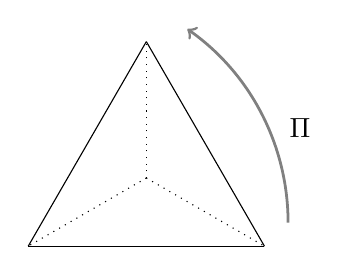
\begin{tikzpicture}[scale=3] \draw (0,0) --
        (1,0); \draw (0,0) -- (1/2,{sqrt(3)/2}); \draw (1/2,{sqrt(3)/2}) --
        (1,0); \draw[dotted] (1/2,{sqrt(3)/6}) -- (1/2,{sqrt(3)/2});
        \draw[dotted] (1/2,{sqrt(3)/6}) -- (0,0); \draw[dotted]
        (1/2,{sqrt(3)/6}) -- (1,0); \node at (1.15,0.5) {$\Pi$}; \draw [line
        width = 1, ->, gray] (1.1,0.1) arc [radius=1, start angle=0, end angle=
        55]; \end{tikzpicture} \label{fig:lookingdown} \end{figure}


    We have rotations $\Pi, \Pi^2$. There are 4 choices from the ``top''
    vertex, so 8 rotations of order 3.

    \underline{View looking down from the perspective on an edge.}
    \begin{figure}[h] \centering 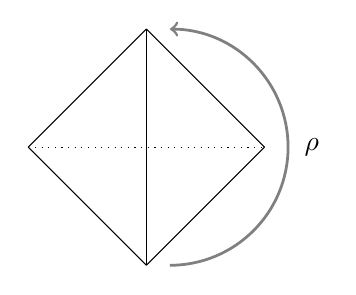
\begin{tikzpicture}[scale=3] \draw (0,0.5) --
        (0.5,1); \draw (1,0.5) -- (0.5,1); \draw (0,0.5) -- (0.5,0); \draw
        (1,0.5) -- (0.5,0); \draw (0.5,1) -- (0.5,0); \draw[dotted] (0,0.5) --
        (1,0.5); \node at (1.2,0.5) {$\rho$}; \draw [line width = 1, ->, gray]
        (0.6,0) arc [radius=0.5, start angle=-90, end angle=90];
      \end{tikzpicture} \label{fig:lookingdownedge} \end{figure}

    Rotation $\rho$ of order 2, one for each pair of opposite edges. So
    elements of order 2.

    The identity rotation makes up the total of 12.  \end{exmp}

  We found 12 rotations of a tetrahedron. Identity rotation and 8 rotations of
  order 3 (2 for each face), and 3 rotations of order 2.

  \textbf{Claim:} The rotations form an group isomorphic to $A_4$.

  \begin{proof} Number the vertices of the tetrahedron $1,2,3,4$. Identify each
    rotation with its effect on the vertex numbers.

    % figure
    \begin{figure}[!tbp] \centering \begin{minipage}[b]{0.4\textwidth}
        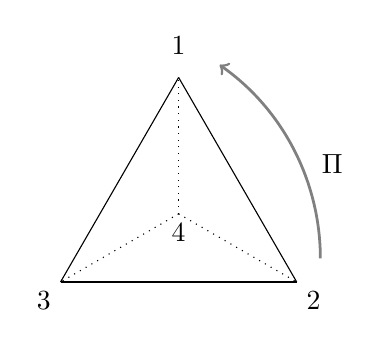
\begin{tikzpicture}[scale=3] \draw (0,0) -- (1,0); \node[below left] at
          (0,0) {3}; \node[below right] at (1,0) {2}; \node at (0.5,1) {1};
          \node[below] at (1/2,{sqrt(3)/6}) {4}; \draw (0,0) --
          (1/2,{sqrt(3)/2}); \draw (1/2,{sqrt(3)/2}) -- (1,0); \draw[dotted]
          (1/2,{sqrt(3)/6}) -- (1/2,{sqrt(3)/2}); \draw[dotted]
          (1/2,{sqrt(3)/6}) -- (0,0); \draw[dotted] (1/2,{sqrt(3)/6}) -- (1,0);
          \node at (1.15,0.5) {$\Pi$}; \draw [line width = 1, ->, gray]
          (1.1,0.1) arc [radius=1, start angle=0, end angle= 55];
        \end{tikzpicture} \end{minipage} \hfill
      \begin{minipage}[b]{0.4\textwidth} \begin{tikzpicture}[scale=3] \draw
          (0,0) -- (1,0); \node[below left] at (0,0) {1}; \node[below right] at
          (1,0) {3}; \node at (0.5,1) {2}; \node[below] at (1/2,{sqrt(3)/6})
          {4}; \draw (0,0) -- (1/2,{sqrt(3)/2}); \draw (1/2,{sqrt(3)/2}) --
          (1,0); \draw[dotted] (1/2,{sqrt(3)/6}) -- (1/2,{sqrt(3)/2});
          \draw[dotted] (1/2,{sqrt(3)/6}) -- (0,0); \draw[dotted]
          (1/2,{sqrt(3)/6}) -- (1,0); \end{tikzpicture} \end{minipage}
      \label{fig:pftriangle} \caption{This rotation corresponds to the
      permutation $(123).$} \end{figure} \begin{figure}[!tbp] \centering
      \begin{minipage}[b]{0.4\textwidth} 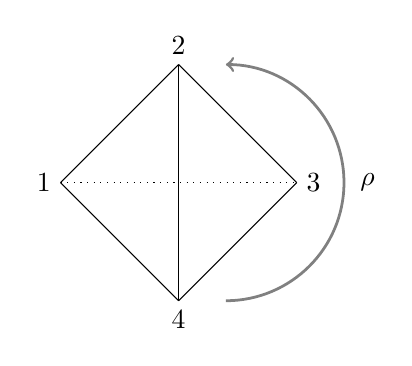
\begin{tikzpicture}[scale=3] \draw
          (0,0.5) -- (0.5,1); \node[left] at (0,0.5) {1}; \node[right] at
          (1,0.5) {3}; \node[above] at (0.5,1) {2}; \node[below] at (0.5,0)
          {4}; \draw (1,0.5) -- (0.5,1); \draw (0,0.5) -- (0.5,0); \draw
          (1,0.5) -- (0.5,0); \draw (0.5,1) -- (0.5,0); \draw[dotted] (0,0.5)
          -- (1,0.5); \node at (1.3,0.5) {$\rho$}; \draw [line width = 1, ->,
          gray] (0.7,0) arc [radius=0.5, start angle=-90, end angle=90];
        \end{tikzpicture} \end{minipage} \hfill
      \begin{minipage}[b]{0.4\textwidth} \label{fig:lookingdownedge} \centering
        \begin{tikzpicture}[scale=3] \node[left] at (0,0.5) {3}; \node[right]
          at (1,0.5) {1}; \node[above] at (0.5,1) {4}; \node[below] at (0.5,0)
          {2}; \draw (0,0.5) -- (0.5,1); \draw (1,0.5) -- (0.5,1); \draw
          (0,0.5) -- (0.5,0); \draw (1,0.5) -- (0.5,0); \draw (0.5,1) --
          (0.5,0); \draw[dotted] (0,0.5) -- (1,0.5); \end{tikzpicture}
      \end{minipage} \label{fig:lookingdownedge} \caption{This rotation
      corresponds to the permutation $(13)(24)$.} \end{figure} Easy to check
    that this gives a bijection between the set of rotations and $A_4$, since
    every rotation is giving an even permutation, and $|A_4|=12$.  Now
    composing rotations is equivalent to composing permutations, so the
    bijection respects multiplication. So the rotations form a group isomorphic
    to $A_4$.  \end{proof}

  There are other symmetries of the tetrahedron, namely reflections.

  Take a plane passing through two vertices, and the midpoint of the edge
  opposite the edge through these two vertices. A reflection through this plane
  is a symmetry of the tetrahedron. 

  Let this reflection be $g$. Let $R$ be the group of rotations. Then $g
  \not\in R$, and so $gR \neq R$. So $G \supseteq R \cup gR$ (where $G$ is the
  symmetry group of the tetrahedron). 

  So $|G| \geq 24$.

  But any symmetry must fix the set of vertices (as a set), and symmetry is
  determined by how it permutes the vertices.

  Since there are only 24 permutations of the vertices, we have $|G|=24$, and
  $G \ism S_4$.  \newpage \subsection{Counting Using Groups} Given an equilateral
  triangle, how many different ways are there of colouring the edges red or
  green? (where colourings which are the same up to rotation or reflection
  count as the same). 

  Possibilities: \begin{itemize} \item All edges red \item Two edges red, one
      green \item One red, two green \item All green \end{itemize} How about a
    more complicated example - say 10 colours available instead of 2. We need a
    technique.

 Idea is: \begin{itemize} \item $\Gamma$ a structure (i.e. a
     triangle/polygon/subset of $\reals^n$).  \item $H$ a group of symmetries
     of $\Gamma$. (Maybe $H$ is not the whole symmetry group.) \item $C$ a set
       of colours.  \end{itemize}

 Apply colours from $C$ to points/lines of $\Gamma$.

 If two colourings $A,B$ satisfy $A=hB$ for some $h \in H$, treat $A$ and $B$
 as the same. Count the total number of colourings.\\

 \begin{definition} If $A$ is a colouring of $\Gamma$, then the set $\left\{ hA
   : h \in H \right\}$ is the \emph{orbit} of $A$ under the action of $H$.\\

   \begin{exmp} $\Gamma$ is an equilateral triangle, $C = \left\{ red, green
     \right\}$, colouring the edges, $H=$ symmetry group $=D_6$.

     $A =$ \begin{figure}[h] \centering 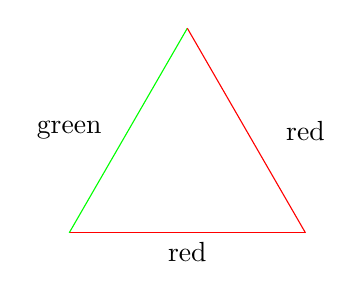
\begin{tikzpicture}[scale=3] \node at
         (0,{sqrt(3)/4}) {green}; \node at (1,{sqrt(3)/4}) {red}; \node[below]
         at (0.5,0) {red}; \draw[red] (0,0) -- (1,0); \draw[green] (0,0) --
         (1/2,{sqrt(3)/2}); \draw[red] (1/2,{sqrt(3)/2}) -- (1,0);
       \end{tikzpicture} \label{fig:lookingdown} \end{figure}

     Orbit of $A = $ \begin{figure}[h] \centering
       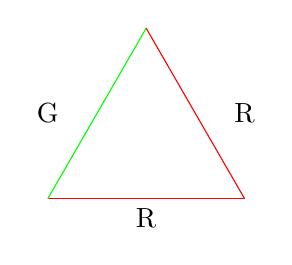
\begin{tikzpicture}[scale=2.5] \node at (0,{sqrt(3)/4}) {G}; \node at
         (1,{sqrt(3)/4}) {R}; \node[below] at (0.5,0) {R}; \draw[red] (0,0) --
         (1,0); \draw[green] (0,0) -- (1/2,{sqrt(3)/2}); \draw[red]
         (1/2,{sqrt(3)/2}) -- (1,0); \end{tikzpicture}\hfill
       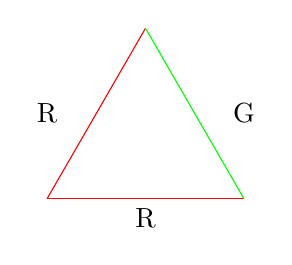
\begin{tikzpicture}[scale=2.5] \node at (0,{sqrt(3)/4}) {R}; \node at
         (1,{sqrt(3)/4}) {G}; \node[below] at (0.5,0) {R}; \draw[red] (0,0) --
         (1,0); \draw[red] (0,0) -- (1/2,{sqrt(3)/2}); \draw[green]
         (1/2,{sqrt(3)/2}) -- (1,0); \end{tikzpicture}\hfill
       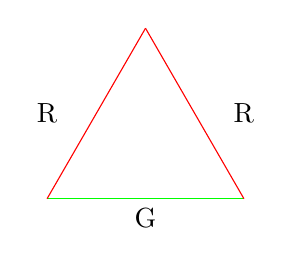
\begin{tikzpicture}[scale=2.5] \node at (0,{sqrt(3)/4}) {R}; \node at
         (1,{sqrt(3)/4}) {R}; \node[below] at (0.5,0) {G}; \draw[green] (0,0)
         -- (1,0); \draw[red] (0,0) -- (1/2,{sqrt(3)/2}); \draw[red]
         (1/2,{sqrt(3)/2}) -- (1,0); \end{tikzpicture} \end{figure}


   \end{exmp} \end{definition} \begin{definition} If $A$ is a colouring of
   $\Gamma$, then the set $\left\{ h \in H : hA=A \right\}$ is the
   \emph{stabilizer} of $A$ in $H$.

   The stabilizer of $A$ is a subgroup of $H$. (Exercise.)\\

   \begin{exmp} $\Gamma, H, A$ as in the examples above.

     Stabilizer of $A$ in $H$ is $\left\{ id,t \right\}$, where $t$ is the
     reflection through the axis $x$.\\ \end{exmp} \end{definition}

 \begin{theorem} Assuming that the group $H$ is finite, we have \[
   \big|\text{Orbit of }A\big| \big|\text{Stabilizer of } A\big|=\big|H\big| \]
   for all colourings $A$.
  
   \label{thm:orbitstabilizer} \end{theorem}

 Recall: We have a structure $S$ (e.g. edges of a polygon, vertices of a
 polygon, etc.) $G$ The symmetry group. $C$ a set of colours. \emph{How many
 colourings of $S$ are possible, if we don't distinguish colourings related by
 a symmetry?}

 Let $\mathcal{A}=$ set of all possible colourings. For $A \in \mathcal{A}$, we
 defined Orbit: $\Orb_G(A)=\left\{ gA : g \in G \right\}$ and Stabiliser:
 $\Stab_G(A) = \left\{ g \in G : gA = A \right\}$ and Orbit-Stabiliser Theorem
 says $|\Orb_G(A)||\Stab_G(A)|=|G|$.

 \begin{proof} (Idea): Suppose $g_1,g_2\in G$ are such that $g_1A=g_2A$. Then
   $g_2^{-1}g_1A=A$, and so $g_2^{-1}g_1A \in \Stab_G(A)$. So
   $g_1\Stab_G(A)=g_2\Stab_G(A)$. Conversely, if $g_1\Stab_G(A)=g_2\Stab_G(A)$
   then $g_1A=g_2A$. So elements of $\Orb_G(A)$ are in bijection with the
   cosets of $\Stab_G(A)$ in $G$. Since the number of cosets is
   $|G|/|\Stab_G(A)|$, we're done.  \end{proof} 

 \begin{exmp} Take $S=$ edges of a square and $G=D_8$ (full symmetry group). $C
   = \left\{ red, green \right\}=\left\{ R,G \right\}$. 
   
   So $A=$ \begin{figure}[h] \centering \begin{tikzpicture}[scale=2]
       \draw[green] (0,0) -- (0,1); \draw[green] (0,0) -- (1,0); \draw[green]
       (1,0) -- (1,1); \draw[red] (0,1) -- (1,1); \draw[dotted] (0,1) -- (1,0);
       \node[below right] at (1,0) {$x$}; \node[below] at (0.5,0) {$G$};
       \node[left] at (0,0.5) {$G$}; \node[right] at (1,0.5) {$G$};
       \node[above] at (0.5,1) {$R$}; \end{tikzpicture}
     \label{fig:coloursquare} \end{figure}
 
 \end{exmp}

  Then orbit is the rotations:

  $\Orb_G(A)=$ \begin{figure}[h] \centering 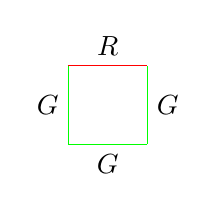
\begin{tikzpicture} \draw[green]
      (0,0) -- (0,1); \draw[green] (0,0) -- (1,0); \draw[green] (1,0) -- (1,1);
      \draw[red] (0,1) -- (1,1); \node[below] at (0.5,0) {$G$}; \node[left] at
      (0,0.5) {$G$}; \node[right] at (1,0.5) {$G$}; \node[above] at (0.5,1)
      {$R$}; \end{tikzpicture}\hfill 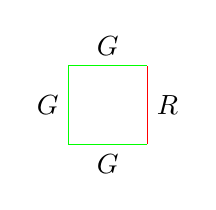
\begin{tikzpicture} \draw[green] (0,0) --
      (0,1); \draw[green] (0,0) -- (1,0); \draw[red] (1,0) -- (1,1);
      \draw[green] (0,1) -- (1,1); \node[below] at (0.5,0) {$G$}; \node[left]
      at (0,0.5) {$G$}; \node[right] at (1,0.5) {$R$}; \node[above] at (0.5,1)
      {$G$}; \end{tikzpicture}\hfill 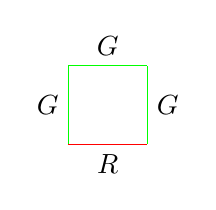
\begin{tikzpicture} \draw[green] (0,0) --
      (0,1); \draw[red] (0,0) -- (1,0); \draw[green] (1,0) -- (1,1);
      \draw[green] (0,1) -- (1,1); \node[below] at (0.5,0) {$R$}; \node[left]
      at (0,0.5) {$G$}; \node[right] at (1,0.5) {$G$}; \node[above] at (0.5,1)
      {$G$}; \end{tikzpicture}\hfill 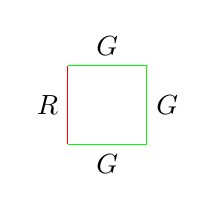
\begin{tikzpicture} \draw[red] (0,0) --
      (0,1); \draw[green] (0,0) -- (1,0); \draw[green] (1,0) -- (1,1);
      \draw[green] (0,1) -- (1,1); \node[below] at (0.5,0) {$G$}; \node[left]
      at (0,0.5) {$R$}; \node[right] at (1,0.5) {$G$}; \node[above] at (0.5,1)
      {$G$}; \end{tikzpicture} \label{fig:coloursquaremult} \end{figure}

   $\Stab_G(A)=\left\{ id, \text{ reflection through }x \right\}$.

   And we have $|\Orb_G(A)||\Stab_G(A)|=4 \times 2 = 8 = |G|$.\\ \begin{lemma}
     (Orbit-Counting, Burnside). The number of orbits of $G$ on colourings is
     \[ \frac{1}{G} \sum_{g \in G}\fix(g) \] Where $\fix(g)$ is the number of
     colourings fixed by $g$.  \label{lem:orbitcounting} \end{lemma}

   \begin{proof} Notice that \begin{align*} \sum_g \fix(g) &= \sum_g |\left\{ A
       : gA = A \right\}| \\ &= |\left\{ (g,A) : g \in G, A \in
         \mathcal{A},gA=A \right\}|\\ &= \sum_{A \in \mathcal{A}}|\left\{ g \in
         G | gA = A \right\}|\\ &= \sum_{A \in \A} |\Stab_G(A)|\\ &= \sum_{A
         \in \A} \frac{|G|}{|\Orb_G(A)|} \end{align*}

so

\begin{align*} \frac{1}{|G|}\sum_{g \in G} \fix(g) = \sum_{A \in \A}
  \frac{1}{\Orb_G(A)}.  \end{align*} But every orbit counts exactly 1 in this
sum since the orbit $O$ has $|O|$ colourings, each counting $\frac{1}{|O|}$. So
$\sum_{A \in \mathcal{A}}\frac{1}{|orb(A)|}$ is the number of orbits.
\end{proof}

\begin{exmps} A necklace has 6 beads, each red or green. How many different
  necklaces are possible?

  Model the necklace as vertices of a regular hexagon.

  The appropriate symmetry group is $D_{12}$ (f h symmetry group). Consider the
  symmetries as permuations of the beads.

  \begin{itemize} \item Rotations: \begin{itemize} \item $id$ fixes all $2^6$
          colourings.  \item $R_\pi = (14)(25)(36)$.  We need $1,4$ the same
          colour etc.  \item $R_\pi$ has 3 cycles, so $2^3$ colourings are
            fixed.

      \item $R_{2\pi/3},R_{4\pi/3}=(135)(246),(153)(264)$.  Both have 2 cycles,
      so fix $2^2$ colourings.  \item $R_{2\pi/6},R_{10\pi/6}=(123456)(165432)$

       Just one cycle, so fix 2 colourings.  \end{itemize}
      

     \item Reflections: Axis through opposite edges (3 reflections)
       $(12)(36)(45)$. 
% fig
       \begin{figure}[h] \centering 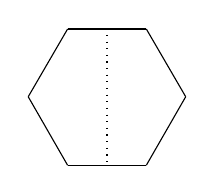
\begin{tikzpicture} \draw[dotted] (1,1.74)
           -- (1,0); \draw (0,0.87) -- (0.5,0); \draw (0.5,0) -- (1.5,0); \draw
           (1.5,0) -- (2,0.87); \draw (2,0.87) -- (1.5,1.73); \draw (1.5,1.73)
           -- (0.5,1.73); \draw (0.5,1.73) -- (0,0.87); \end{tikzpicture}

         \label{fig:necklace1} \end{figure}
      
       
       3 cycles, so $2^3$ fixed colourings. 
% fig
Axis through opposite vertices (3 reflections) $(13)(2)(46)(5)$.

       \begin{figure}[h] \centering 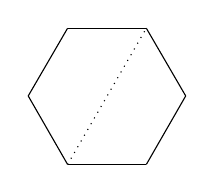
\begin{tikzpicture} \draw[dotted] (0.5,0)
           -- (1.5,1.73); \draw (0,0.87) -- (0.5,0); \draw (0.5,0) -- (1.5,0);
           \draw (1.5,0) -- (2,0.87); \draw (2,0.87) -- (1.5,1.73); \draw
           (1.5,1.73) -- (0.5,1.73); \draw (0.5,1.73) -- (0,0.87);
         \end{tikzpicture}

         \label{fig:necklace1} \end{figure}
       

       4 cycles. so $2^4$ fixed colourings.

       
       Now the Orbit-Counting lemma gives

       \begin{align*} \# \text{orbits} &= \frac{1}{12}(64 + 8 + 2\times4 +
         2\times 2 + 3 \times 8 + 3 \times 16)\\ &= \frac{1}{12}\times 156 \\
         &= 13.  \end{align*} \end{itemize} \end{exmps}

\section{Linear Algebra} \subsection{Determinants} We know determinants for $2
\times 2$ matrices: \[ \begin{vmatrix} a & b \\ c & d \end{vmatrix} = ad - bc
\] And $3 \times 3$ matrices: \[ \begin{vmatrix} a & b & c \\ d & e & f \\ g &
    h & i \end{vmatrix} = a \begin{vmatrix} e & f \\ h & i \end{vmatrix} -
b\begin{vmatrix} d & f \\ g & i \end{vmatrix} + c\begin{vmatrix} d & e \\ g & h
\end{vmatrix} = aei - afh - bdi +bfg +cdh-ceg.  \]

Let $A=(a_{ij})$  be an $n \times n$ matrix.

Write $A_{ij}$ for the minor obtained by deleting the $i^{th}$ row and the
$j^{th}$ column. We could define $\det A$ (or $|A|$ ) by analogy with the $3
\times 3$ case, as

\[ |A| = a_{11}|A_{11}| - a_{12}|A_{12}| + a_{13}|A_{13}| \cdots +
(-1)^{n-1}a_{1n}|A_{1n}|.  \]

(Definition by expansion alog the first row.)

This is a \emph{recursive} definition -- $n \times n$ determinants are defined
in terms of $(n-1) \times (n-1)$ determinants.

Expanding along a different row (or a column) would give the same result (proof
later)


In fact we will use an alternative definition.

The terms in \[ \begin{vmatrix} a & b & c \\ d & e & f \\ g & h & i
\end{vmatrix} \]

are each a product of three entries, one from each row and column.

Suppise we pick the entry in column $f(i)$ from row $i$, then $f$ is a
permutation of $\left\{ 1,2,3 \right\}$. So the terms correspond to elements of
$S_3$.

\begin{align*} aei &\leftrightarrow \text{id} \\ bfg &\leftrightarrow (123) \\
  cdh &\leftrightarrow (132) \\ -bdi &\leftrightarrow (12) \\ -cdg
  &\leftrightarrow (13) \\ -afh &\leftrightarrow (23).  \end{align*} Notice the
sign before each term is just the signature of the corresponding permutation.

Similarly for the $2 \times 2$ determinant: $\begin{vmatrix}a & b \\ c &
  d\end{vmatrix}$

\begin{align*} ad &\leftrightarrow \text{id} \\ -bc &\leftrightarrow (12).
\end{align*}

\begin{definition} Let $A$ be an $n \times n$ matrix, $A = (a_{ij})$. The
  determinant of $A$ is \[ \det A = \sum_{\sigma \in S_n} \sgn(\sigma)
  a_{1\sigma(1)}a_{2\sigma (2)}\dots a_{n \sigma (n)}.  \] \end{definition}

\begin{proposition} \label{prp:swaprows} Suppose that $B$ is obtained from $A$
  by swapping two rows. Then I claim $\det B = -\det A$.  \end{proposition}

  \begin{proof} Suppose that rows $p$ and $q$ are the rows that are going to be
    swapped. Let $A=(a_{ij}),B=(b_{ij})$. I claim that we can write \[ b_{ij} =
    a_{\tau (i) j}, \quad\text{where }\tau = (pq) \quad (2-\text{cycle}).\]

      \begin{align*} \det B &= \sum_{\sigma \in S_n} \sgn(\sigma)
        b_{1\sigma(1)}b_{2\sigma (2)}\dots b_{n \sigma (n)}\\ &= \sum_{\sigma
        \in S_n} \sgn(\sigma) a_{\tau(1)\sigma(1)}a_{\tau(2)\sigma (2)}\dots
        a_{\tau(n) \sigma (n)}\\ &= \sum_{\sigma \in S_n} \sgn(\sigma)
        a_{1\tau^{-1}\sigma(1)}a_{2\tau^{-2}\sigma (2)}\dots a_{n\tau^{-n}
      \sigma (n)} \end{align*} (Same $n$ factors in each product, but in a
    different order). Notice that $\tau = \tau^{-1}$.  \begin{align*} &=
      \sgn{\tau} \sum_{\sigma \in
      S_n}\sgn(\tau)\sgn(\sigma)a_{1\tau\sigma(1)}\dots a_{n \tau\sigma(n)} \\
      &= - \sum_{\sigma \in S_n}\sgn(\tau\sigma)a_{1\tau\sigma(1)}\dots a_{n
      \tau\sigma(n)} \\ &= - \sum_{\tau\sigma \in
      S_n}\sgn(\tau\sigma)a_{1\tau\sigma(1)}\dots a_{n \tau\sigma(n)}
    \end{align*} Since the sum is over all group elements in either case.
    \begin{align*} &= -\det A.  \end{align*} \end{proof}

  \begin{proposition}\hfill \label{prp:rowssame} \begin{itemize} \item If $A$
          has an all-0 row, then $\det A=0$.  \item If $A$ has two rows the
          same then $\det A=0$.  \item If $A$ is triangular (upper or lower)
            then $\det A=a_{11}a_{22}\dots a_{nn}$ \end{itemize}


  \end{proposition}

  \begin{proof} Suppose that $A$ has all $0$s in row $i$. Then
    $a_{i\sigma(i)}=0$ for all $\sigma \in S_{n}$. So $a_{1\sigma(1)}\dots
    a_{n\sigma(n)}=0$, for all $\sigma$.

    So $\det A = 0$.

    Suppose that $A$ has rows $p$ and $q$ the same. Let $B$ be the matrix
    obtained from $A$ by exchanging rows $p$ and $q$. Then $\det B=-\det A$ by
    Prop \ref{prp:swaprows}.  But clearly $B=A$, so $\det A = - \det A$. So
    $\det A=0$.

    Let $\sigma$ be a non-identiy permutation in $S_n$. There must exist $i,j
    \in \left\{ 1,\dots n \right\}$ with $\sigma(i) > i, \sigma(j)<j$. Whether
    $A$ is upper-or-lower-triangular, one of $a_{i\sigma(i)}$ or
    $a_{j\sigma(j)}$ is 0. So $a_{1\sigma(1)}\dots a_{n\sigma(n)}=0$, and so
    the only $\sigma \in S_n$ which contributes to the $\det A$ is the
    identity.

    Hence $\det A = \sgn(\id)a_{11}\dots a_{nn}$ and $\sgn(\id)=+1$, giving the
    result. 

  \end{proof} \begin{proposition} (Row operations).  \begin{enumerate} \item
          Let $B$ be obtained by swapping two rows. Then $\det B=-\det A$.
        \item Let $B$ be obtained from $A$ by multiplying a row by a scalar
          $\lambda$.

          Then $\det B = \lambda \det A$.  \item Let $B$ be obtained from $A$
            by adding $\lambda$ times row $i$ to row $j$, where $i \neq j$.
            Then $\det B = \det A$.  \end{enumerate} \end{proposition}
    \begin{proof}\hfill \begin{enumerate} \item $(i)$ Suppose that $A$ has all
            0s in row $i$. Then $a_{i\sigma(i)} = 0$ for all $\sigma \in n$.
          So $a_{1\sigma(1)}\dots a_{n\sigma(n)} = 0$, for all $\sigma$. So
        $\det A = 0$.  \item  Suppose that $A$ has rows $p$ and $q$ the same.
          Let $B$ be the matrix obtained from $A$ by exchanging rows $p$ and
          $q$. Then $\det B = -\det A $ (Proposition \ref{prp:swaprows}.) But
          clearly $B = A$, so $\det A = -\det A$. So $\det A = 0$.

     \item Let $\sigma$  be a non-identity permutation. There must exist $i, j
       \in \left\{ 1,\dots ,n \right\}$ with $\sigma(i) > i$ and $\sigma(j) <
       j$. Whether $A$ is upper or lower triangular, one of $a_{i\sigma(i)}$ or
       $a_{j\sigma(j)}$ is 0. So $a_{1\sigma(1)}\dots a_{n\sigma(n)} = 0$, for
       all non-identity $\sigma$’s, and so the only $\sigma \in S_n$ which
       contributes to $\det A$ is the identity. Hence $\det A = \sgn(\id)
       a_{11}\dots a_{nn}$. And $\sgn(\id) = +1$, giving the result.
   \end{enumerate} \end{proof}

\begin{proposition}\hfill \label{prp:rowops} \begin{enumerate} \item Let $B$ be
        obtained from $A$ by swapping two rows. Then $\det B = - \det A$.
      \item Let $B$ be obtained from $A$ by multiplying a row by a scalar
        $\lambda$. Then $\det B = \lambda\det A$.  \item Let $B$ be obtained
          from $A$ by adding $\lambda$ times row $i$ to row $j$ $(i \neq j)$.
          Then $\det B = \det A$.  \end{enumerate} \end{proposition}

\begin{proof}\hfill \begin{enumerate} \item This is Proposition
        \ref{prp:swaprows}.  \item Suppose we multiply row $p$ by scalar
          $\lambda$. So \[ b_{ij} = \begin{cases} \lambda a_{ij}, & \text{if }
              i=p \\ a_{ij}, & \text{otherwise} \end{cases} \] For $\sigma \in
            S_n$ we have \begin{align*} b_{1\sigma(1)}\dots b_{n\sigma(n)} &=
              a_{1\sigma(1)}\dots \lambda a_{p\sigma(p)}\dots a_{n \sigma(n)}
              \\ &= \lambda (  a_{1\sigma(1)}\dots  a_{n\sigma(n)} )
            \end{align*} So \begin{align*} \sum_\sigma \sgn (\sigma)
              b_{1\sigma(1)}\dots b_{n\sigma(n)} &= \lambda \sum_\sigma
              \sgn(\sigma)  a_{1\sigma(1)}\dots a_{n\sigma(n)}\\ \implies \det
              B &= \lambda \det A \end{align*} \item We have $b_{ij} = a_{jk} +
              \lambda_{ik}$ for all $k$ Also, $b_{kk}=a_{kk}$ is $k \neq j$. We
              have, for $\sigma \in S_n$,

      \begin{align*} b_{1\sigma(1)}\dotsb_{n\sigma(n)} &= a_{1 \sigma(1)} \dots
        ( a_{j \sigma(j)} + \lambda  a_{i \sigma(j)} ) \dots a_{n\sigma(n)} \\
        &= \elemt{a}{1} \dots \elemt{a}{j} \dots\elemt{a}{n} + \elemt{a}{1}
        \dots \lambda a_{i\sigma(j)} \dots a_{n\sigma(n)} \end{align*} It
      follows that

      \[ |B| = |A| + \lambda \begin{vmatrix} a_{11} & \cdots & a_{1n}\\ \vdots
          &        & \vdots \\ a_{i1} & \cdots & a_{1n} \\ \vdots &        &
          \vdots \\ a_{i1} & \cdots & a_{in} \\ \vdots &        & \vdots \\
          a_{n1} & \cdots & a_{nn} \\ \end{vmatrix} \] And this is 0 since the
        matrix on the right has two rows the same (Prop. \ref{prp:rowssame}).
    \end{enumerate} \end{proof}

\begin{exmp} What is the determinant of \[ \left(\begin{matrix} 1 & 2 & 2 & 0
    \\ 1 & 4 & 0 & 3 \\ -1 & 0 & -2 & 3 \\ 1 & 0 & 8 & -6 \end{matrix}\right)
\] Use row operations. By Prop. \ref{prp:rowops} we have \begin{align*} |A| =
  \begin{vmatrix} 1 & 2 & 2 & 0 \\ 1 & 4 & 0 & 3 \\ -1 & 0 & -2 & 3 \\ 1 & 0 &
    8 & -6 \end{vmatrix} &= \begin{vmatrix} 1 & 2 & 2 & 0 \\ 0 & 2 & -2 & 3 \\
    0 & 0 & 2 & 0 \\ 0 & 0 & 4 & -3 \end{vmatrix}\\ &= \begin{vmatrix} 1 & 2 &
    2 & 0 \\ 0 & 2 & -2 & 3 \\ 0 & 0 & 2 & 0 \\ 0 & 0 & 0 & -3 \end{vmatrix}\\
  &= -12 \end{align*}

\end{exmp}

\begin{proposition}
  \label{prp:detab} Suppose that $B$ can be obtained from $A$ by row
operations: \begin{enumerate} \item Exchanging rows \item Scaling rows by
    non-zero scalar \item Adding multiples of one-row to another row.
  \end{enumerate} Then $\det B = 0 \iff \det A = 0$.  \end{proposition}

\begin{proof} Clear from Prop. \ref{prp:rowops}.  \end{proof}

\begin{proposition} \label{prp:dettran} Let $A$ be an $n\times n$ matrix. Then
  $|A| = |A|^T$  (where $A^T$ is the \emph{transpose} of $A$.)
\end{proposition}

\begin{proof} Let $A^T = (b_{ij})$. Then $b_{ij} = a_{ji}$. Let $\sigma \in
  S_n$. We have \begin{align*} \elemt{b}{1} \dots \elemt{b}{n} &=
    a_{\sigma(1)1} \dots a_{\sigma(n)n} \\ &= a_{1\sigma^{-1}(1)}\dots a_{n
      \sigma^{-1}(n)} \end{align*}

So 

\[ \det A^T = \sum_{\sigma in S_n}\sgn(\sigma)  a_{1\sigma^{-1}(1)}\dots a_{n
\sigma^{-1}(n)} \] Now summing over all $\sigma$ is equivalent to summing over
$\sigma^{-1}$ and $\sgn(\sigma) = \sgn(\sigma^{-1})$

\begin{align*} &= \sum_{\sigma^{-1} \in S_n}\sgn
  (\sigma^{-1})a_{1\sigma^{-1}(1)}\dots a_{n \sigma^{-1}(n)}\\ &= \det A
\end{align*} \end{proof} Proposition \ref{prp:dettran}  implies that all of our
results concerning rows and row operations also hold for columns / column
operations (since columns of $A$ are the rows of $A^T$).

\subsection*{Expansion along rows / columns} Let $A = (a_{ij} )$, and let
$A_{ij}$ be the minor obtained by deleting row $i$ and column $j$. Then

\textbf{Claim:} \[ \det A = \sum_{j=1}^n (-1)^{i+j}a_{ij}|A_{ij}|, \quad
\text{for any } i \]

\begin{proof} First suppose $i = 1$. We have from the definition that $|A|$ is
  a sum over all elements $\sigma \in S_n$. Consider all $\sigma$ such that
  $\sigma(1) = 1$. It's not hard to see that

  \[ \sum_{\sigma(1)=1}\sgn(\sigma)a_{11}a_{2\sigma(1)}\dots a_{n\sigma(n)} =
  a_{11}|A_{11}| \]

  How about $\sigma$ such that $\sigma(1) = 2$? Let $B$ be obtained from $A$ by
  swapping columns 1 and 2. Then \[ B = \begin{vmatrix} a_{12} & a_{11} &
      \cdots & a_{1n} \\ a_{22} & a_{21} & \cdots & a_{2n} \\ \vdots & \vdots &
      & \vdots  \\ a_{n2} & a_{n1} & \cdots & a_{nn} \end{vmatrix} \] So terms
    of $\det A$ corresponding to $\sigma(1) = 2$ are the same as the terms of
    $b_{11}|B_{11}|$. But swapping two columns negates the determinant, so \[
      \sum_{\sigma(1)=2}\sgn (\sigma) a_{12}a_{2\sigma(2)} \dots a_{n\sigma(n)}
      = -b_{11}|B_{11}| = -a_{12}|A_{12}| \] \end{proof} 
    
    \[
    A = \left( 
    \begin{matrix}
      a_{11} & a_{12} & \dots & a_{1n} \\
      \vdots &        &       & \vdots \\
      a_{n1} & a_{n2} & \dots & a_{nn}
    \end{matrix}
    \right)
  \]
  \[
    B = \left( 
    \begin{matrix}
      a_{12} & a_{11} & \dots & a_{1n} \\
      \vdots &        &       & \vdots \\
      a_{n2} & a_{n1} & \dots & a_{nn}
    \end{matrix}
    \right)
    \]

   ($A$ with columns 1 and 2 swapped)

   We have $|B| = -|A|$ (prop \ref{prp:swaprows}

   If $\sgn(\sigma)a_{1\sigma(1)}\dots a_{n\sigma(n)}$ is a term of $|A|$, 
   then $-\sgn(\sigma)a_{1\sigma(1)\dots a_{n\sigma(n)}}$ 
   must be a term in $|B|$.

   We know that the terms of $|B|$ including $b_{11}=a_{12}$ are
   given by $b_{11}|B_{11}| = a_{12}|A_{12}|$.

   Hence the terms of $|A|$ including $a_{12}$ are given by  $-a_{12}|A_{12}|$.

   How about the terms of $|A|$ including $a_{13}$? 
   Bring the $3^{rd}$ columns to the front, without changing the order
   of the columns. Do this by first swapping columns 1 and 3, then 2 and 3.

   (Note $(123)=(23)(13)$.)
   
   If $B$ is the resulting matrix then 
   $|B|=|A|$ (Since we've swapped columns twice.)

   \[
   B = \left( 
   \begin{matrix}
     a_{13} & a_{11} & a_{12} & \dots & a_{1n} \\
     \vdots &        &        &       & \vdots \\
     a_{n3} & a_{n1} & a_{n2} & \dots & a_{nn}
   \end{matrix}
   \right)
   \]
  

   The  terms of $|B|$ including $a_{13}$ are given $a_{13}|A_{13}|$. So
   these are the terms of $|A|$ too.

   Continue in this way. Since bringing column $j$ to the front induces a $j-$
   cycle, we get $|B|=(-1)^{j+1}|A|$. So we end up with 
   \begin{align*}
     |A| &= a_{11}|A_{11}| - a_{12}|A_{12}| + a_{13}|A_{13}| - \dots\\
     &= \sum_{j=1}^n (-1)^{j+1}a_{ij}|A_{ij}|.
   \end{align*}
   This accounts for expansion along the $1^{st}$ row.

   How about expanding along row $i$?

   We can do this by first bringing row $i$ to the top without changing the
   order of the other rows.

   This induces an $i-$cycle on the rows, which can be done by swapping
   rows $i-1$ times.

   So if $B$ is the resulting matrix, then $|B|=(-1)^{i-1}|A|$.

   So we get

   \begin{align*}
     |A| &= (-1)^{i-1} \sum_{j=1}^n (-1)^{j+1} a_{ij} |A_{ij}| \\
     &= \sum_{j=1}^n (-1)^{i+j} a_{ij} |A_{ij}|.
   \end{align*}

   \begin{remark}
     We can also find determinants by expansion along columns. (By Prop. \ref{prp:dettran}).
   \end{remark}
  
   \begin{proposition}
     Let $A$ be an $n\times n$ matrix.
     The following statements are equivalent. 
     \begin{enumerate}
       \item $|A| \neq 0$.
       \item $A$ is invertible.
       \item The system of equations $A\underline{x}=\underline{0}$ has no 
         solutions except $\underline{x}=\underline{0}$.
       \item $A$ can be reduced to $I$ by row operations.
     \end{enumerate}
   \end{proposition}

   \begin{proof}
     $(2) \iff (3) \iff (4)$ from $M1GLA$.
     \begin{itemize}
       \item[$(4) \iff (1)$] Suppose $I$ can be obtained from $A$. by row
         operations. We know $|I|\neq 0$ and so $|A|\neq 0$, by Prop.
         \ref{prp:detab}.

       \item[$(1)\iff (4)$] Let $A_{ech}$ be the row echelon form of $A$.
         Then $A_{ech}$ is obtained from $A$ by row operations.

         So if $|A|\neq 0$ then $|A_{ech}| \neq 0$.

         So $A_{ech}$ has no all$-0$ rows.

         Hence $A_{ech}$ can be transferred to $I$ by row operations.
     \end{itemize}
   \end{proof}

   The last major property of determinants that we want is $\Det{AB} =
   \Det{A}\Det{B}$. For this we require:

   \subsubsection*{Elementary Matrices}

   \[
     A_{i}(\lambda) = \left( 
     \begin{matrix}
       1 &        & & & & \\
         & \ddots & & & & \\
         &        & 1 & & & \\
         &        &   & \lambda & & \\
         &        &   &         & \ddots & \\
         &        &   &         &        & 1 \\
     \end{matrix}
     \right)
   \]
   $\lambda \neq 0$, $I$ with row $i$ scaled by $\lambda$.

  \[
    B_{ij} = \left( 
    \begin{matrix}
     1 &  & & & & &  \\
      & \ddots & & & & & \\
      & & 0 & & 1 & &  \\
      & & &  \ddots & &  & &  \\
      & & 1 & & 0 & &  \\
      &  & & & & \ddots & \\
      &  & & & & &1  \\
    \end{matrix}
    \right)
  \]
  $i \neq$ j, $I$ with rows $i$ and $j$ swapped.

  \[
    C_{ij}(\lambda) = \left( 
    \begin{matrix}
      1 &        &         &  \\
        & \ddots & \lambda &  \\
        &        &         & 1
    \end{matrix}
    \right)
  \]

    $i \neq j$, $\lambda \neq 0$. $I$ with $\lambda$ times row $j$ added to 
    row $i$.

    The elementary matrices correspond to elementary row operations.

    If $M$ is an $n \times n$ matrix with rows $r_1,\dots r_n$ then:

    Multiplying row $r_i$ by $\lambda$ $\rightarrow$ $A_i(\lambda)M$

    Swapping rows $r_i$ and $r_j$ $\rightarrow$ $B_{ij}M$

    Adding $\lambda r_j$ to $r_i$ $\rightarrow$ $C_{ij}(\lambda)M$.\\

    \begin{exmps}
  $A_2(3) = \left( 
\begin{matrix}
  1 & 0 \\
  0 & 3
\end{matrix}
  \right)$.

  \begin{align*}
  \left( 
  \begin{matrix}
    1 & 0 \\
    0 & 3
  \end{matrix}
  \right)\left( 
  \begin{matrix}
    p & q \\
    r & s
  \end{matrix}
  \right) = \left( 
  \begin{matrix}
    p & q \\
    3r & 3s
  \end{matrix}
  \right)
\end{align*}

  For $
    B_{12} = \left( 
  \begin{matrix}
    0 & 1 \\
    1 & 0
  \end{matrix}
  \right)
$

\begin{align*}  
\left( 
  \begin{matrix}
    0 & 1\\
    1 & 0
  \end{matrix}
  \right)\left( 
  \begin{matrix}
    p & q \\
    r & s
  \end{matrix}
  \right) = \left( 
  \begin{matrix}
    r & s \\
    p & q
  \end{matrix}
  \right)
\end{align*}

For $
  C_{12}(3) = \left( 
  \begin{matrix}
    1 & 3 \\
    0 & 1
  \end{matrix}
  \right)
$

  \begin{align*}
  \left( 
  \begin{matrix}
    1 & 3 \\
    0 & 1
  \end{matrix}
  \right)\left( 
  \begin{matrix}
    p & q \\
    r & s
  \end{matrix}
  \right) = \left( 
  \begin{matrix}
    p + 3r & q + 3s \\
    r & s
  \end{matrix}
  \right).
\end{align*}

We observe that

\begin{align*}
  \Det{A_i(\lambda)} &= \lambda \\
    \Det{B_{ij}} &= -1\\
    \Det{C_{ij}(\lambda)} &= 1
\end{align*}

(Since all of these are obtained by applying an elementary row operation to $I$.)

So we have $\Det{EM}=\Det{E}\Det{M}$ whenever $E$ is an elementary matrix,
by Prop. \ref{prp:rowops}
\end{exmps}


\end{document}

